%%____________________________________________________________________________||
\section{Validation with the \alphat analysis}
The \alphat analysis is an inclusive search for supersymmetry which
uses a fine categorisation in \nj,\nb,\scalht,and \mht to provide
sensitivity to a wide range of new physics models. The results 
of this search for 12.9\fb of data at 13TeV from Run 2 of the LHC
are described fully in \cite{CMS-PAS-SUS-16-016}. In this section,
the use of aggregate regions is discribed for the \alphat analysis, as well as a 
validation of the simplified likelihood method.

\subsection{Application of the the aggregate regions with the \alphat analysis}

The final \nj,\nb categories and \scalht binning used for the full likelihood 
are summarised in Table~\ref{tab:binning}. These bins are further split into
$100 \GeV$ \mht bins as defined in \cite{alphaT}. The control region
predictions are inclusive in \mht but binned according to Table~\ref{tab:binning}.

\begin{table}[htb!]
  \topcaption{Summary of the lower bounds of the first and final bins
    in \scalht (the latter in parentheses) as a function of \njet and
    \nb. Intermediate \scalht bins are taken from 200,250,300,400,500,600,700,$>800\GeV$} 
  \label{tab:binning}
  \centering
  \footnotesize
  \begin{tabular}{ lrrrr }
    \hline
%    \njet                   & \multicolumn{4}{c}{\nb}                                           \\
%    \cline{2-5}
%                            & 0         & 1         & 2         & $\geq$3                       \\
    $\njet \backslash\, \nb$ & 0         & 1         & 2         & $\geq$3                       \\
    \hline
    \multicolumn{5}{l}{\bf Monojet}                                                              \\
    1                        & 200 (600) & 200 (500) & -     & -                         \\
    \multicolumn{5}{l}{\bf Asymmetric}                                                           \\
    2                        & 200 (600) & 200 (500) & 200 (400) & -                         \\
    3                        & 200 (600) & 200 (600) & 200 (500) & 200 (300)                     \\
    4                        & 200 (600) & 200 (600) & 200 (600) & 250 (400)                     \\
    $\geq$5                  & 250 (600) & 250 (600) & 250 (600) & 300 (500)                     \\
    \multicolumn{5}{l}{\bf Symmetric}                                                            \\
    2                        & 200 (800) & 200 (800) & 200 (600) & -                         \\
    3                        & 200 (800) & 250 (800) & 250 (800) & \phantom{0}-\phantom{0} (250) \\
    4                        & 300 (800) & 300 (800) & 300 (800) & 300 (800)                     \\
    $\geq$5                  & 350 (800) & 350 (800) & 350 (800) & 350 (800)                     \\
    \hline
  \end{tabular}
\end{table}

The $\mathcal{O}800$ bins provide generic sensitivity but are not optimal
for simple reinterpretation. A simplification can be made that maintains
sensitivity to a large class of models through the use of aggregate regions.
The final categories are shown in Table~\ref{tab:agg-binnning}. In addition
for each aggregate category eight exclusive \mht bins with
lower bounds $100,200,300,400,500,600,700,\ge800GeV$ are defined.

\begin{table}[tb]
  \topcaption{Aggregate region bins. The \scalht dimension is
  merged to $\geq200\GeV$, \nb to two categories of \nb = $0,1$ and $\geq2$. 
  The merged \nj~ categories are summarised in this table. Each category is
  further binned using eight \mht bins with lower bounds from $100-800\GeV$.}
  \label{tab:agg-binning}
  \centering
  \footnotesize
  \begin{tabular}{ llll }
    \hline
    \nj topology & \multicolumn{3}{l}{Merged jet categories} \\
    \hline
     & \bf Monojet & \bf Asymmetric& \bf Symmetric \\
    Monojet-like & 1 & 2 & 2                         \\
    Asymmetric high \nj& - & 3, 4, $\geq5$ & -                 \\
    Mid \nj & - &  3, 4 & -                        \\
    High \nj & - & $\geq5$ & -                     \\
    \hline
  \end{tabular}
\end{table}

The jet categories are merged to four seperate categories motivated by their sensitivity to 
different new physics topologies. For example, the Monojet-like topology is targeted towards
dark matter models and compressed spectra while the high \nj topology targets 
uncompressed gluino and squark models.
The b-jet categories are combined as $\nb=0,1$ \nb models and $\nb\geq2$ targeted at
light and heavy flavour new physics respectively. Finally, the \scalht dimension is 
entirely merged as the \mht dimension is strongly correlated with \scalht and
can be used to provide similar sensitivity. The use of the
aggregate regions ensures that the components of the background are still
corrected based on the nominal, finely binned regions with relevant systematics.

\subsection{Results using aggregate regions for the \alphat analysis}

When using the full likelihood presenting the final fit results is
a signifcant issue. The large number of bins makes understanding any possible trends,
excesses or deficits in the fit result across the signal region difficult. 
The aggregate regions can be used to rapidly find global features in the fit result as
the full picture can be summarised, in the case of the \alphat analysis, 
in eight \mht distributions as shown in Fig.~\ref{fig:aggFitResult}. These
show the predictions using the fit to the control regions only compared to 
the data observations. Post signal region fit results are shown in Appendix~\ref{app:}.

To evaluate the effect on the sensitivity the expected and observed 95\% upper limit
on the signal strength, defined as in \cite{limit-stuff}, for the full signal region 
is compared that using the aggregate regions. The limits are shown side by side
in Fig~\ref{fig:limit-planes} for three models, T2tt T2bb and T1bbbb. Where the mass
splittings are small the expected limits typically reduce by $\mathcal{O} 100\GeV$ 
compared to the full signal region for all models  

The aggregate fit result considering only the control regions, 
can be used to provide predictions and uncertainties
to allow recasters to interpret their own models. In the case of the \alphat search
this is significantly easier than recasting the full signal region. To make best use of this information, 
as will be discussed in Section~\ref{sec:simplified-likelihood}, 
the covariance matrix encoding the level of correlation between bins must also be utilised.
\clearpage
\begin{figure}[!tbhp]
    \caption{ Signal region predictions and data observations for the aggregate regions. 
    The predictions are made using a fit to the control region only. \label{fig:aggFitResult} }
  \begin{center}
    \subfigure[Monojet-like, $\nb = 0$]{ 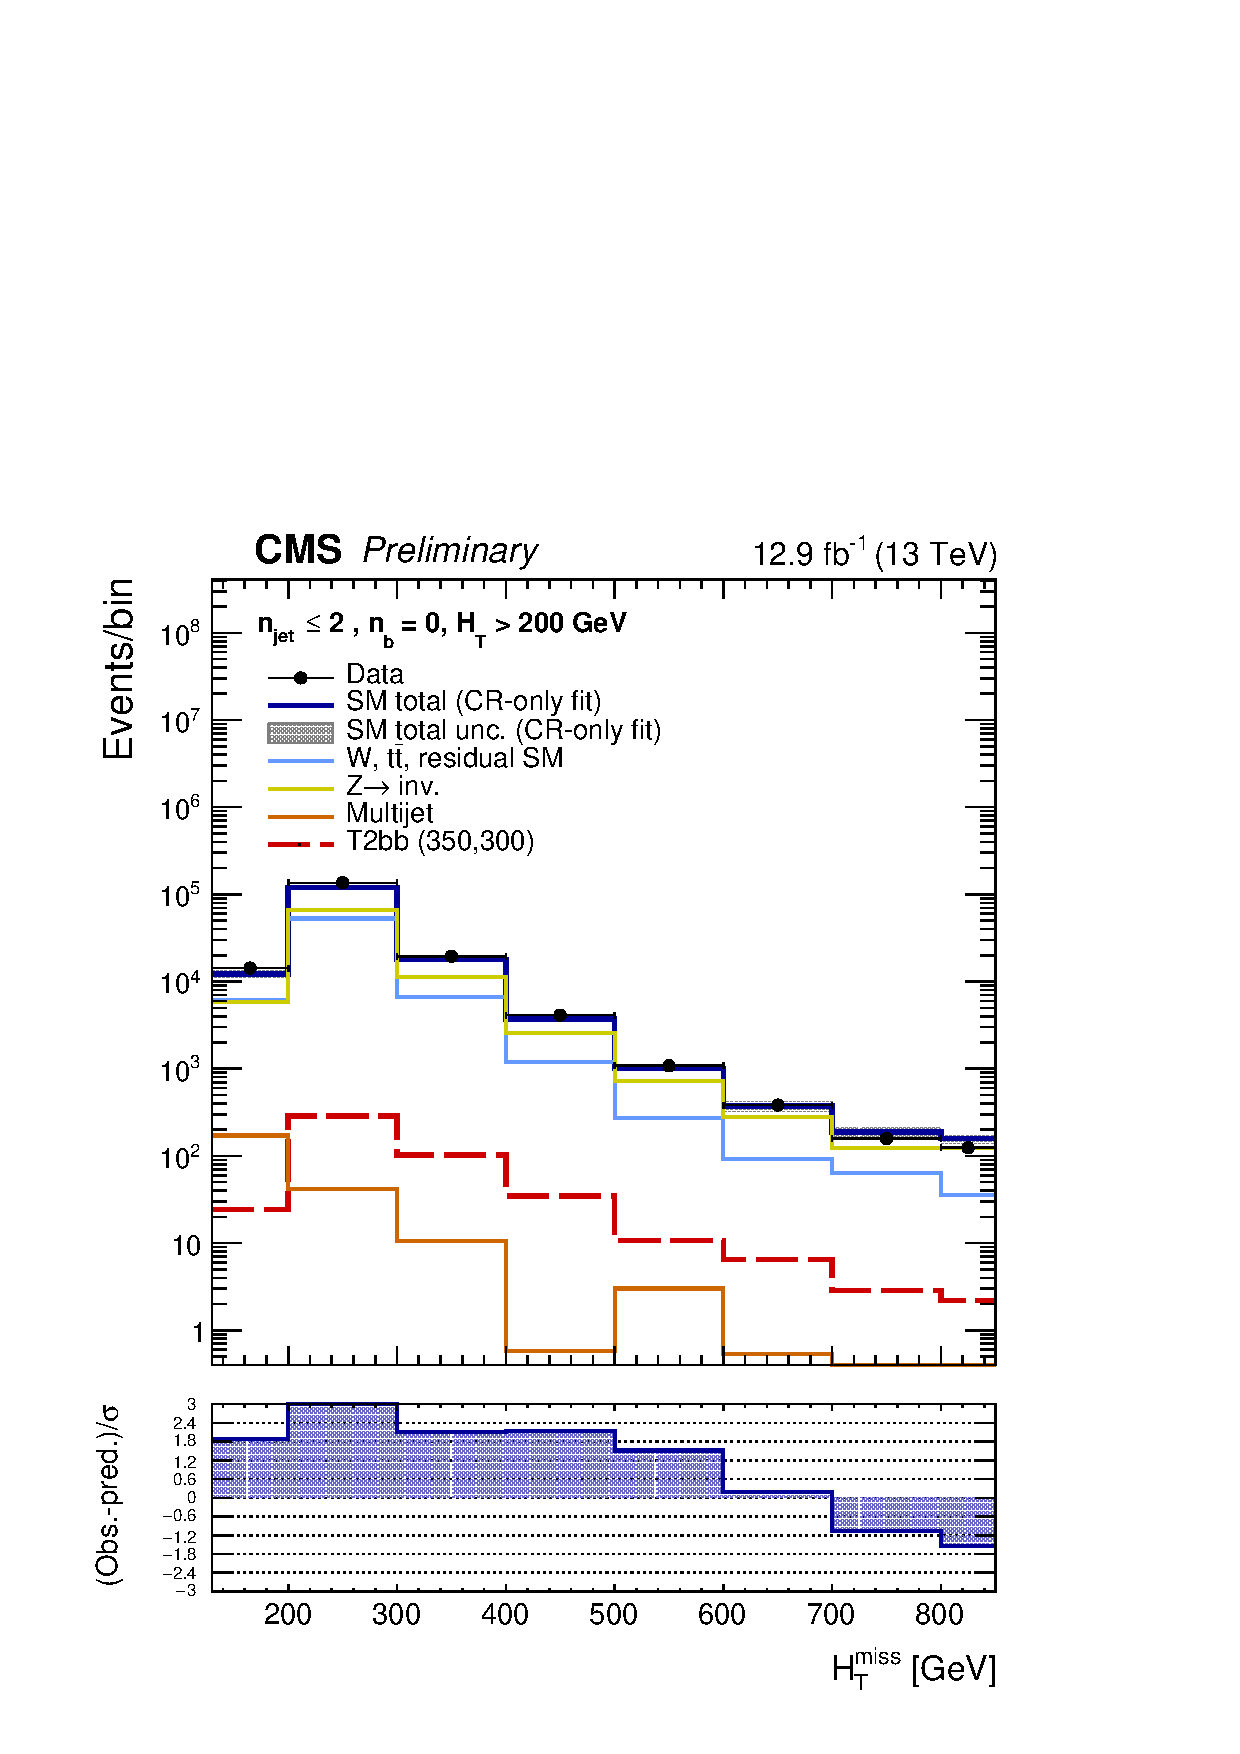
\includegraphics[width=0.4\textwidth]{figures/alphaT/agg_fitResults/mhtShape_eq0b_le2j_200_Inf_crfit_aux.pdf} } ~~
    \subfigure[Monojet-like, $\nb \geq 1$]{ 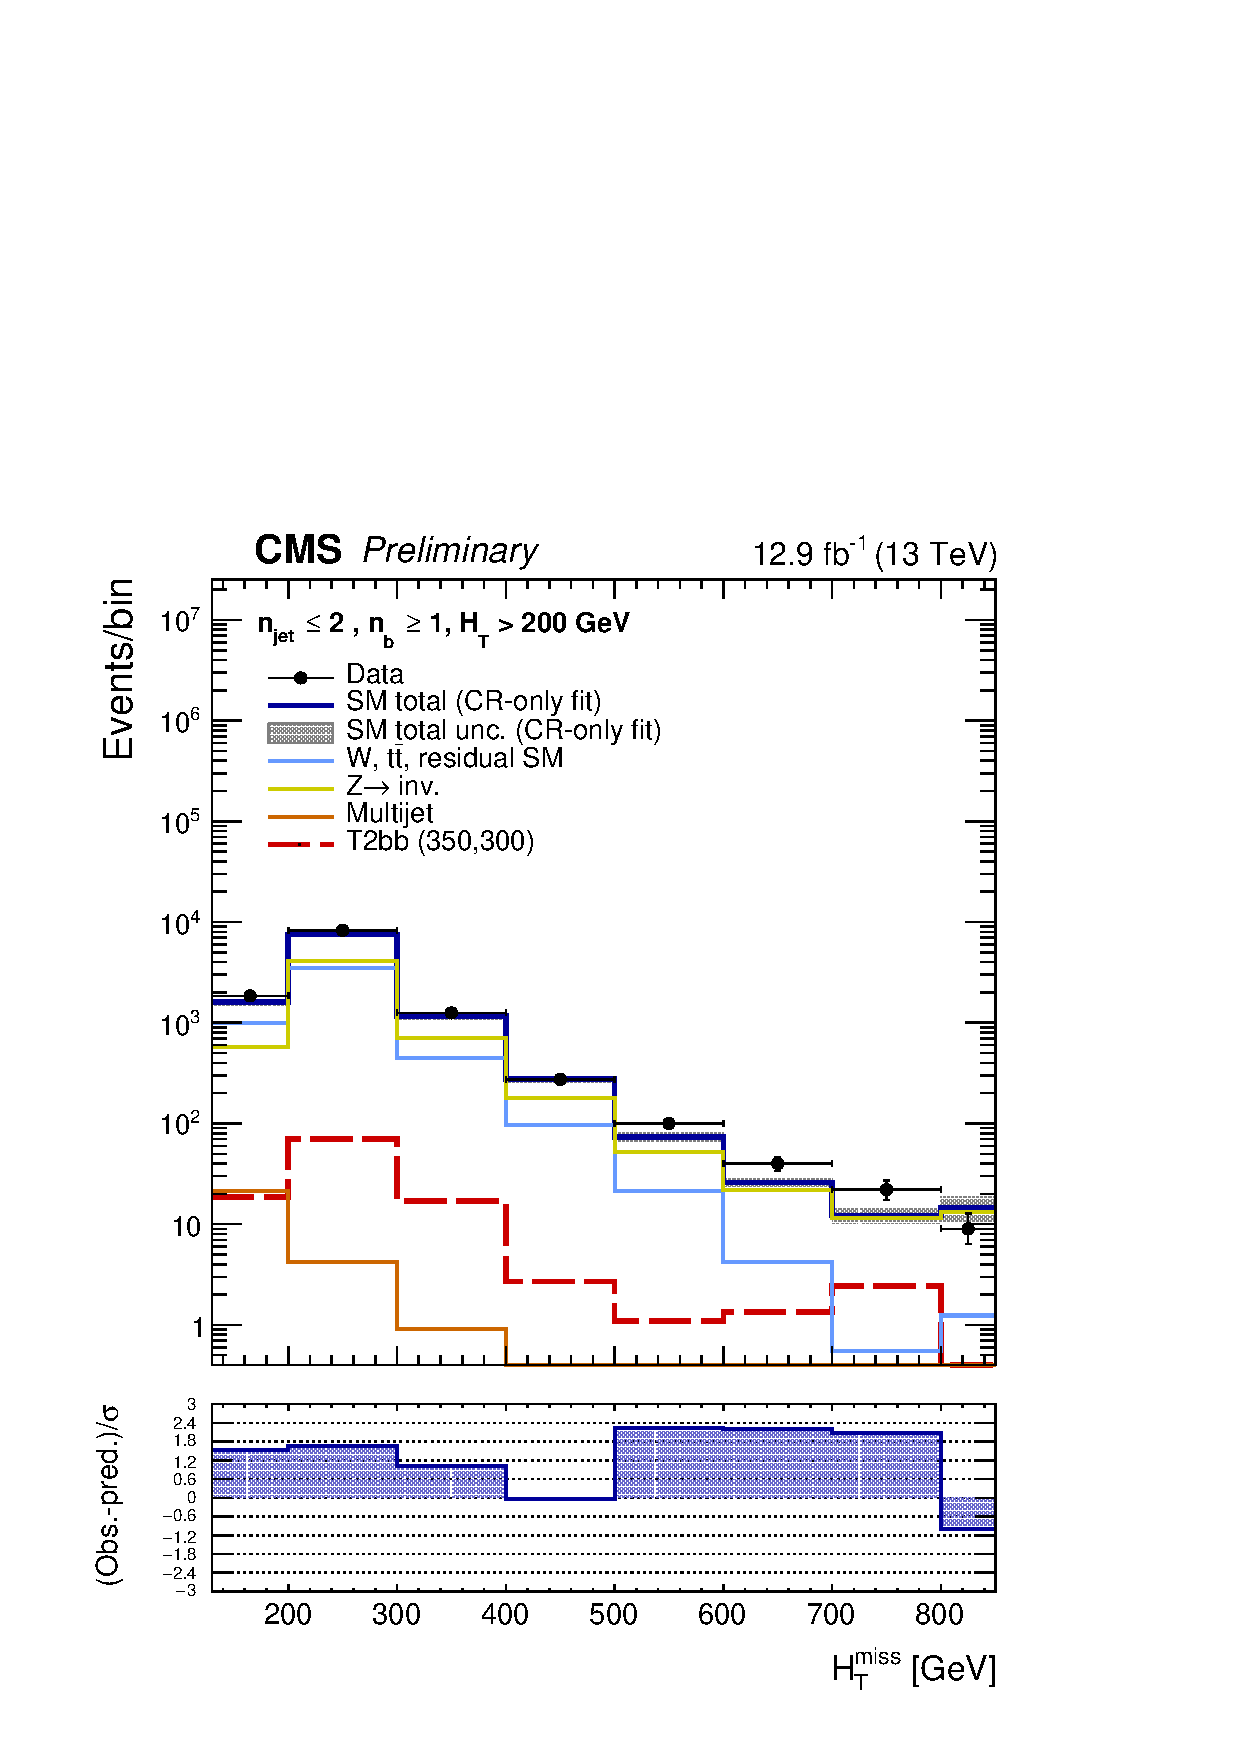
\includegraphics[width=0.4\textwidth]{figures/alphaT/agg_fitResults/mhtShape_ge1b_le2j_200_Inf_crfit_aux.pdf} } \\
    \subfigure[Asymmetric high \nj, $\nb \leq 1$]   { 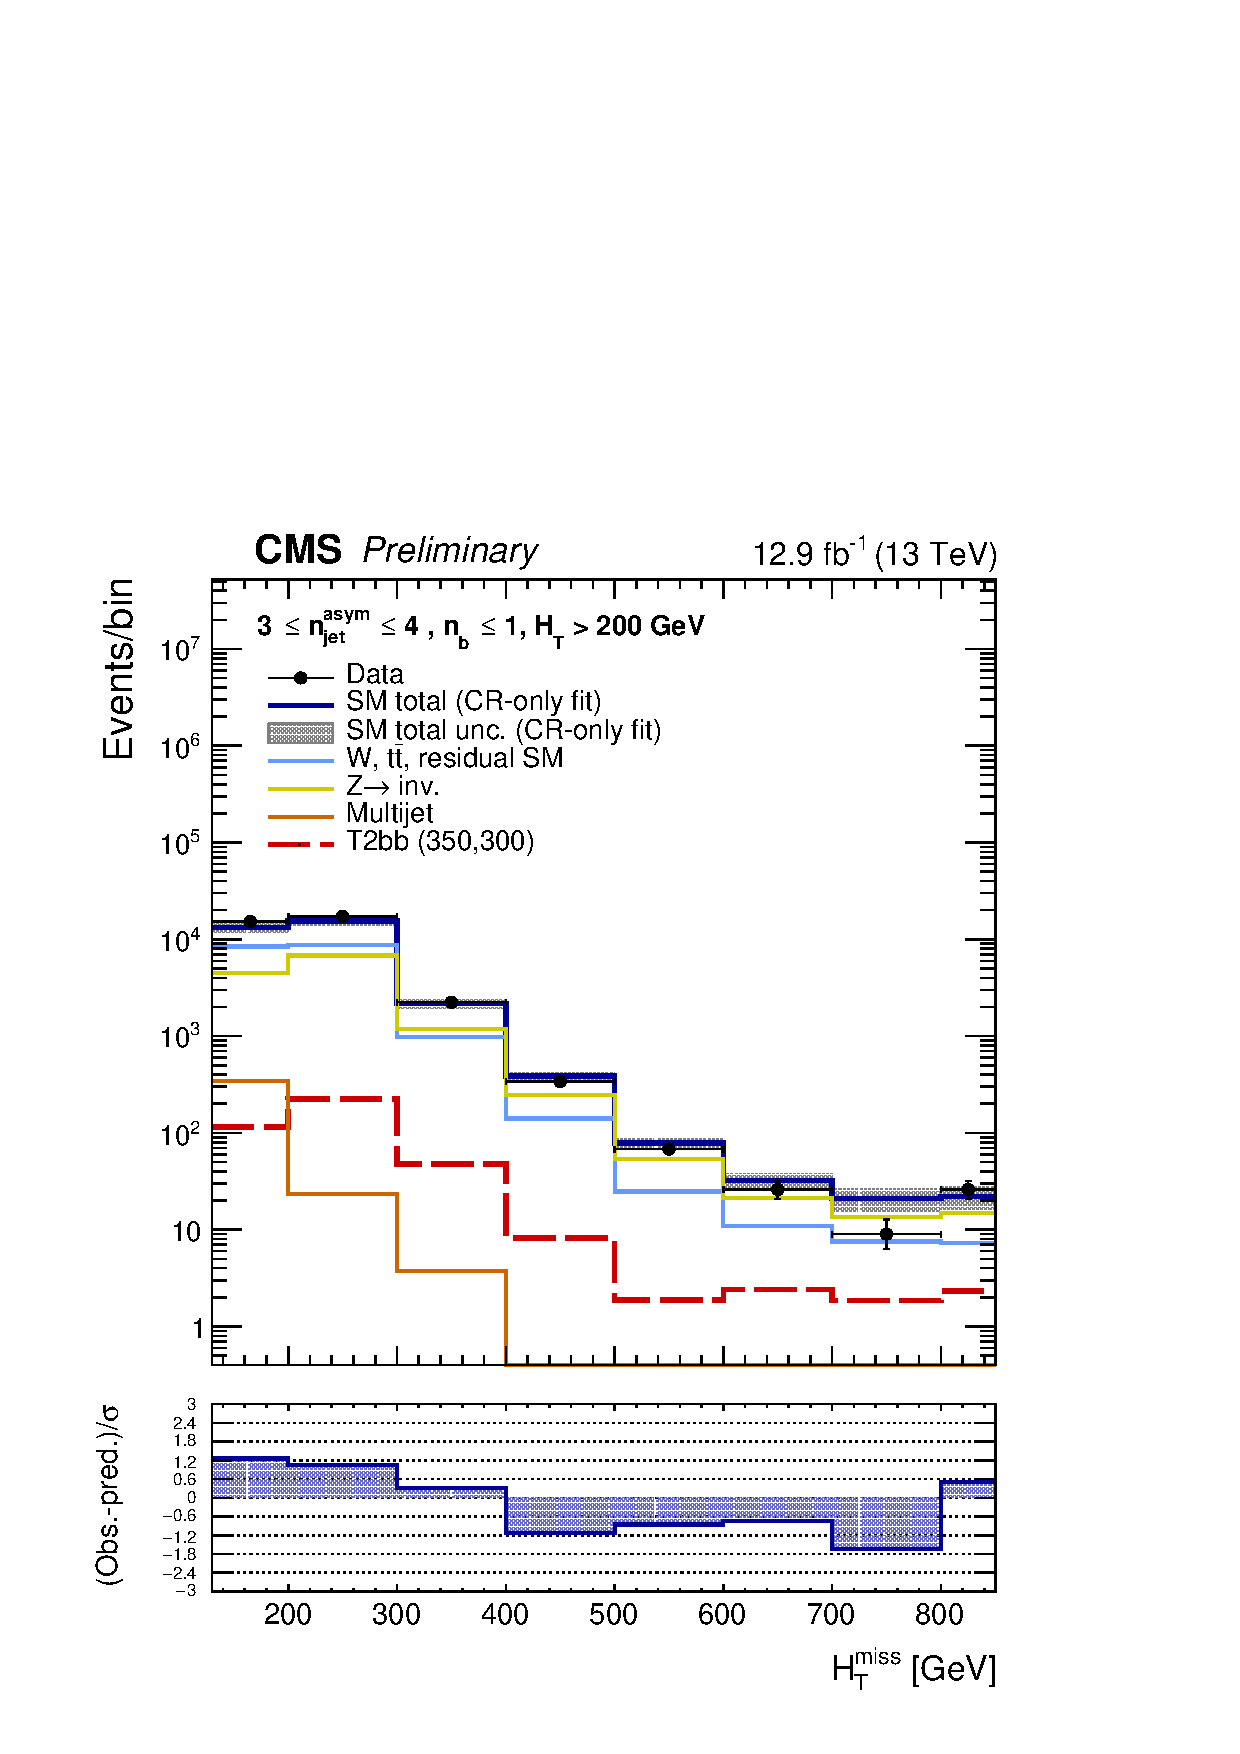
\includegraphics[width=0.4\textwidth]{figures/alphaT/agg_fitResults/mhtShape_le1b_ge3a_200_Inf_crfit_aux.pdf} } ~~
    \subfigure[Asymmetric high \nj, $\nb \geq 2$]{ 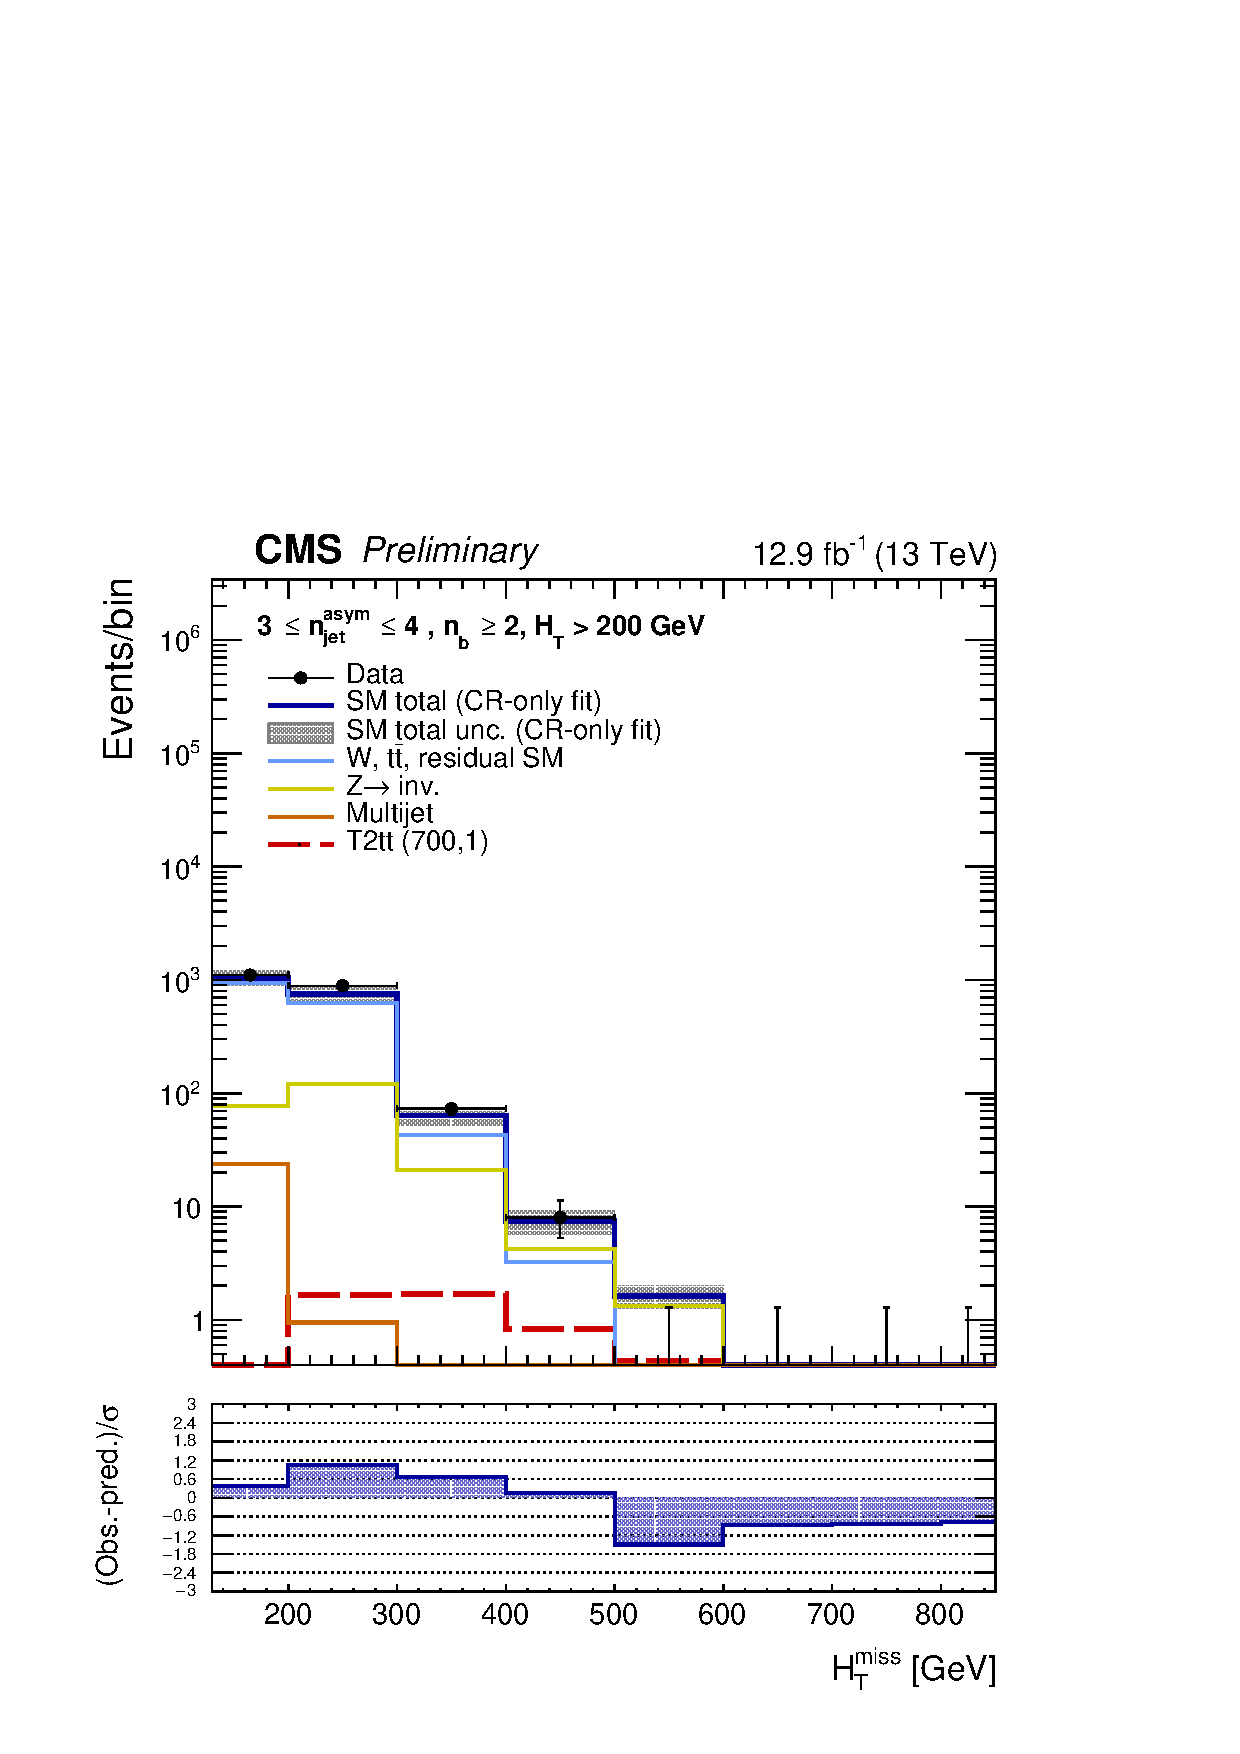
\includegraphics[width=0.4\textwidth]{figures/alphaT/agg_fitResults/mhtShape_ge2b_ge3a_200_Inf_crfit_aux.pdf} } \\
    \subfigure[Mid \nj, $\nb \leq 1$]   { 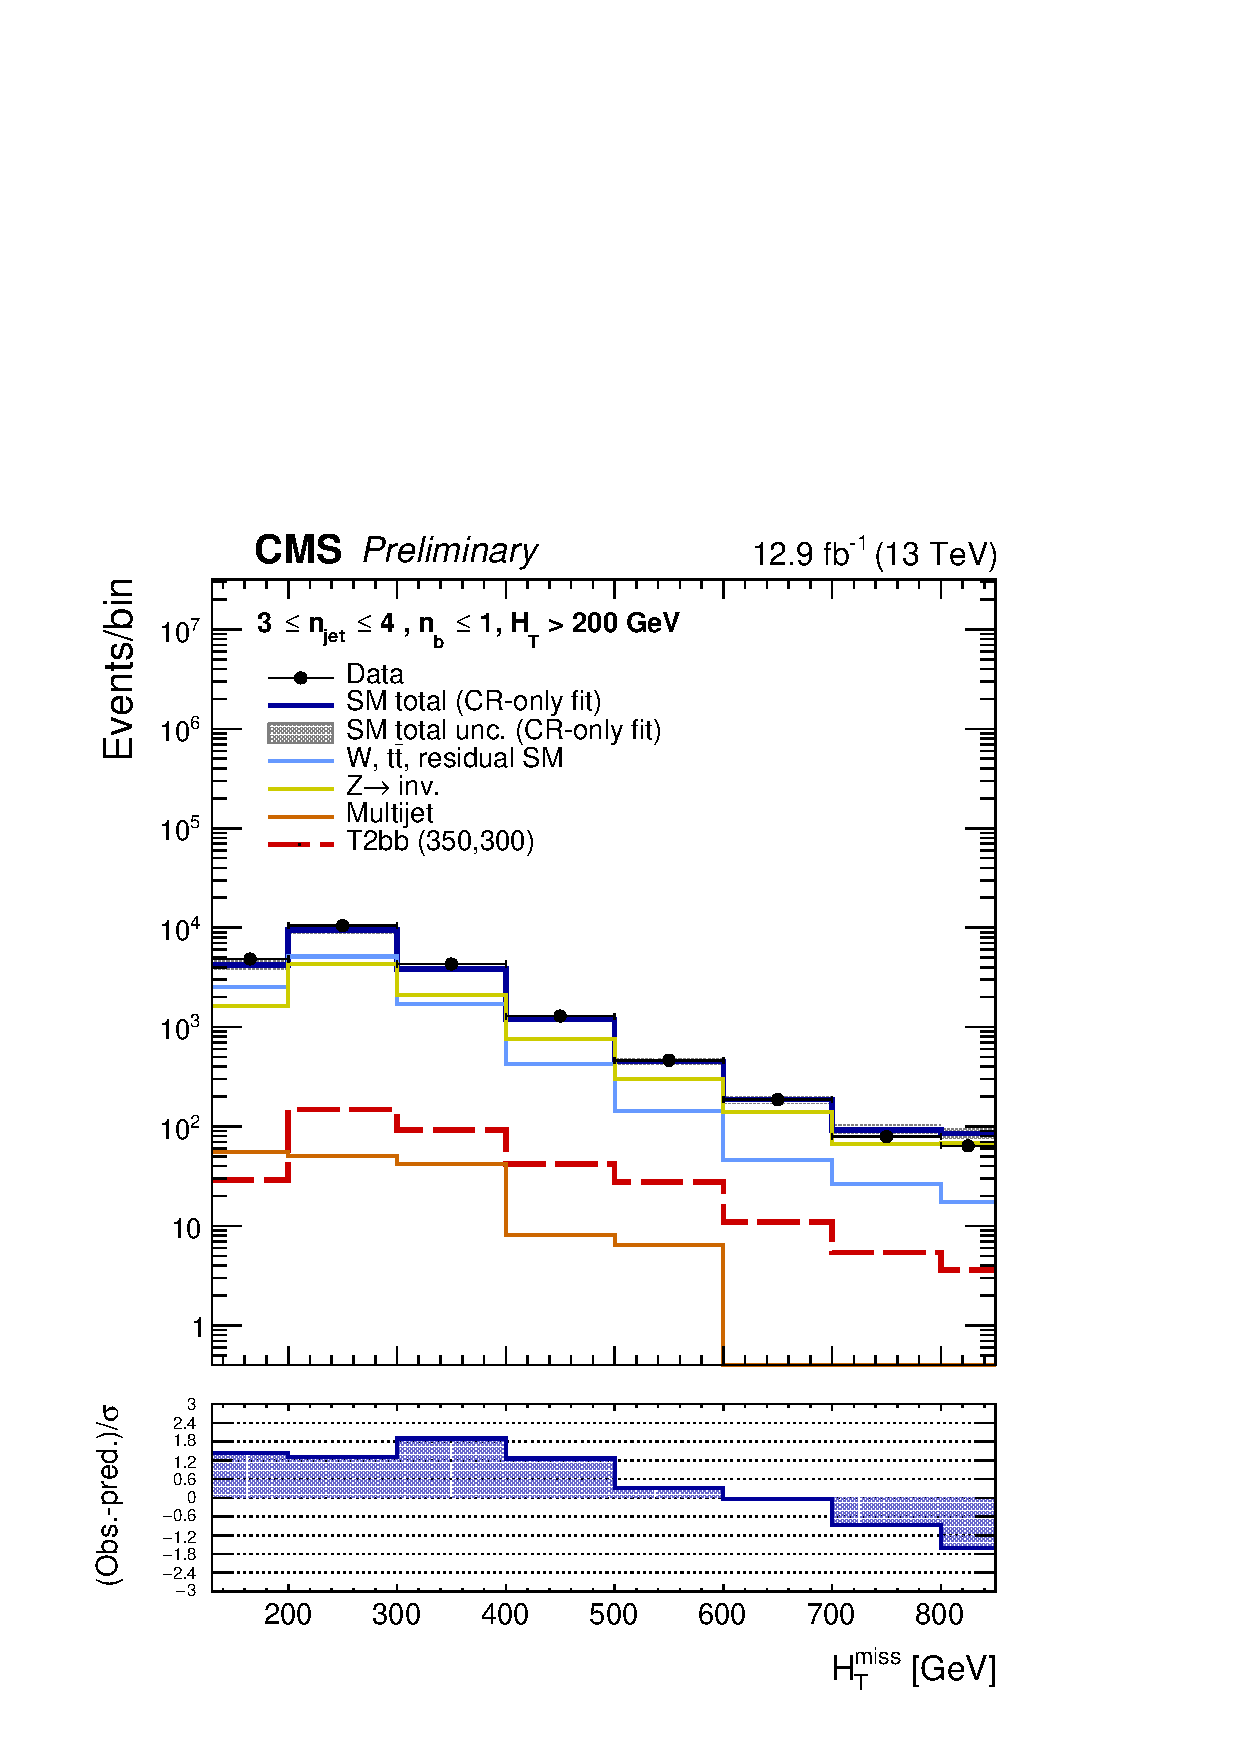
\includegraphics[width=0.4\textwidth]{figures/alphaT/agg_fitResults/mhtShape_le1b_ge3j_200_Inf_crfit_aux.pdf} } ~~
    \subfigure[Mid \nj, $\nb \geq 2$]{ 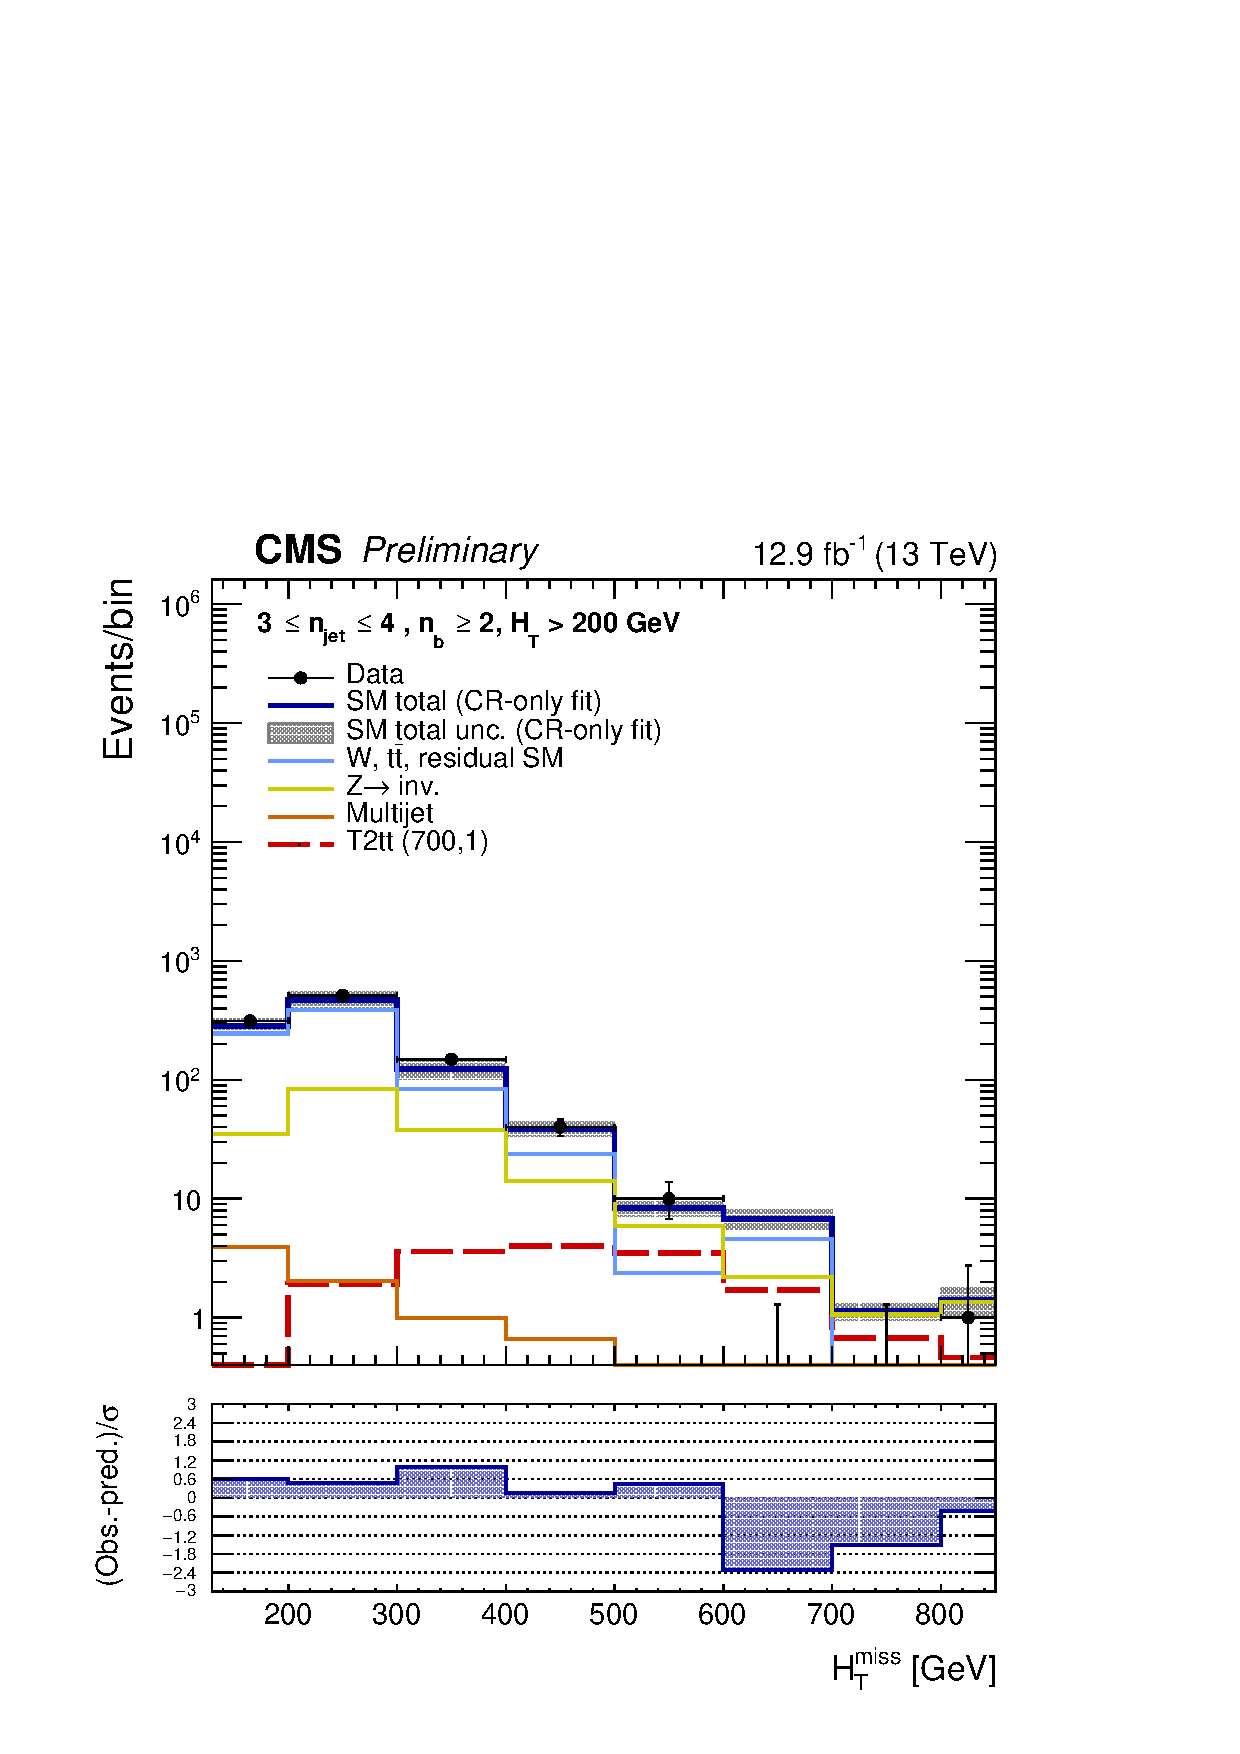
\includegraphics[width=0.4\textwidth]{figures/alphaT/agg_fitResults/mhtShape_ge2b_ge3j_200_Inf_crfit_aux.pdf} } \\
    \subfigure[High \nj, $\nb \leq 1$]   { 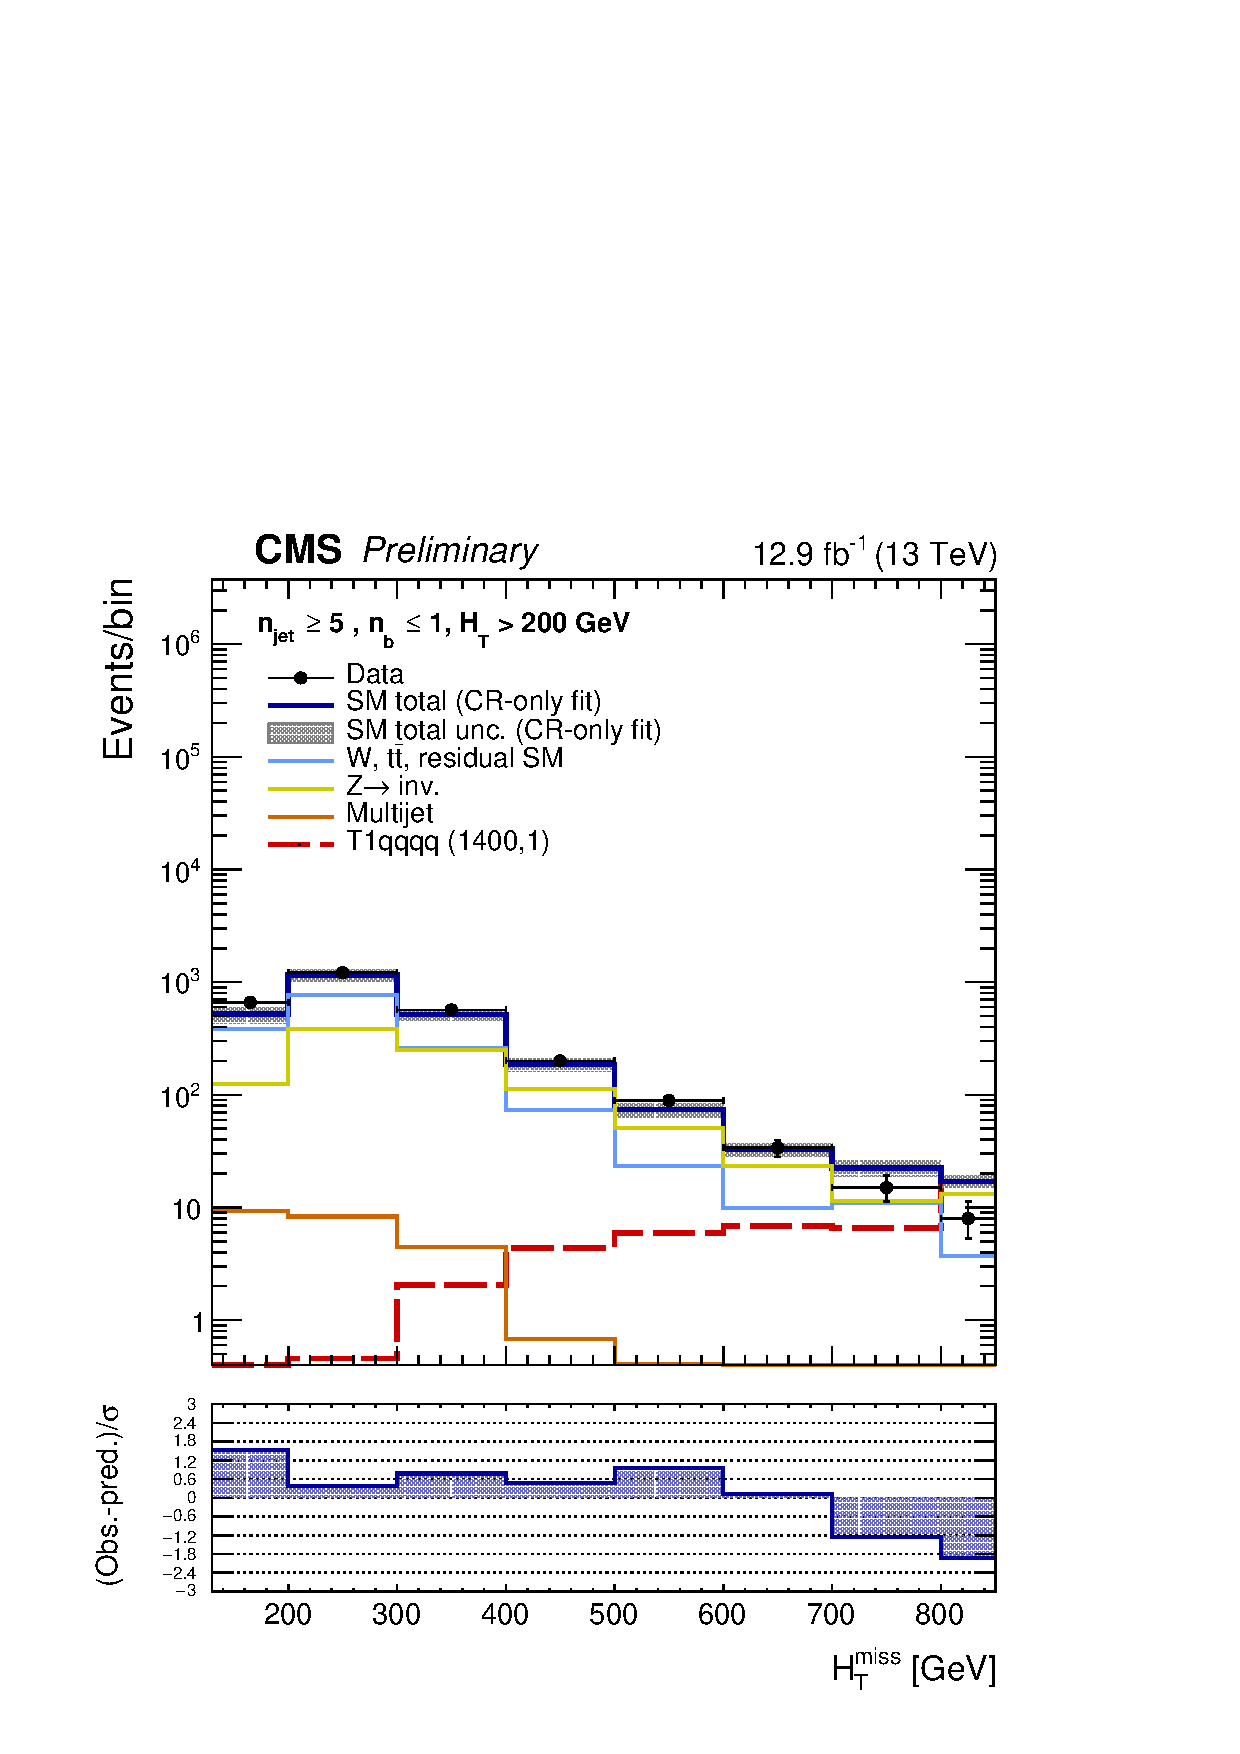
\includegraphics[width=0.4\textwidth]{figures/alphaT/agg_fitResults/mhtShape_le1b_ge5j_200_Inf_crfit_aux.pdf} } ~~
    \subfigure[High \nj, $\nb \geq 2$]{ 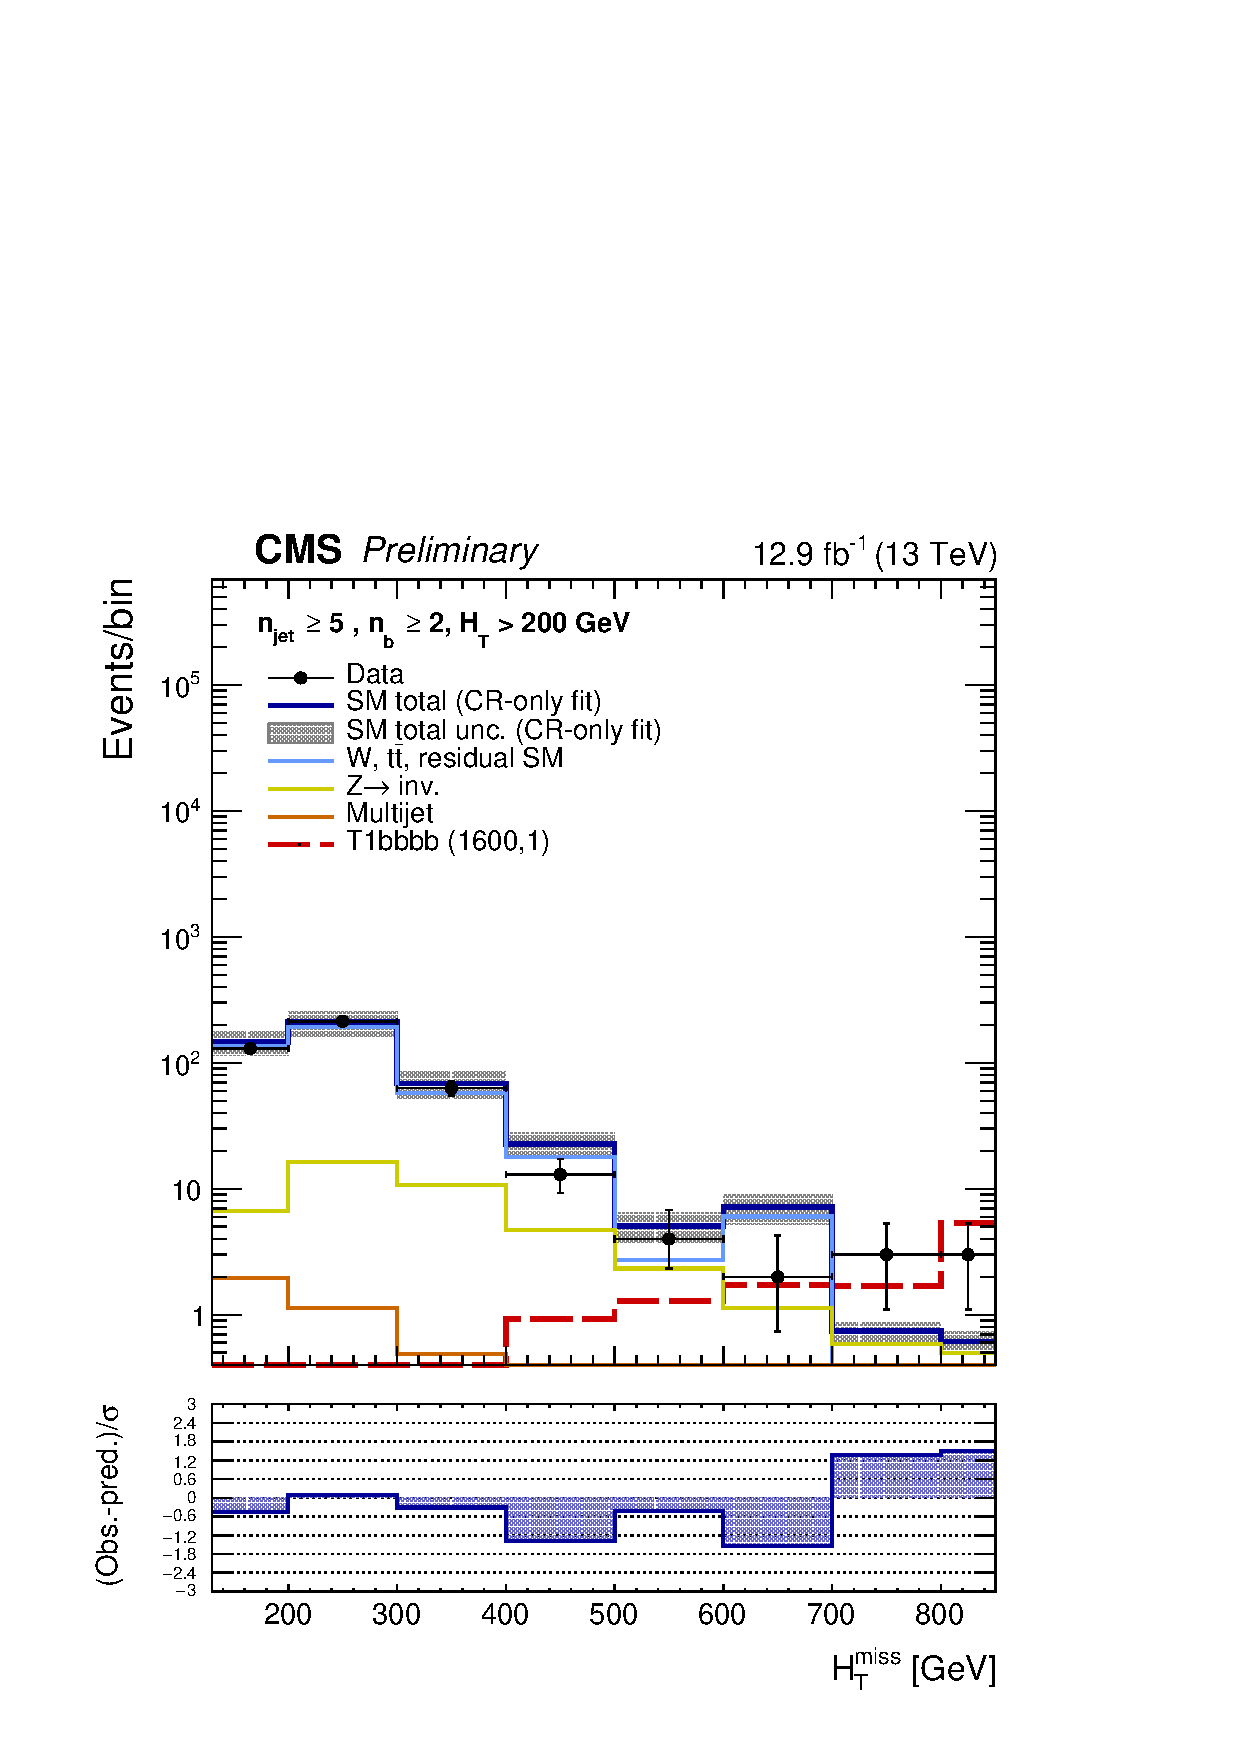
\includegraphics[width=0.4\textwidth]{figures/alphaT/agg_fitResults/mhtShape_ge2b_ge5j_200_Inf_crfit_aux.pdf} } \\
  \end{center}
\end{figure}


\clearpage
\begin{figure}[!tbhp]
    \caption{ Limit planes shown for both the full signal regions (left) and the aggregate regions (right).\label{fig:limit-planes}. 
    For the compressed models. }
  \begin{center}
    \subfigure[T2bb full signal region]{ 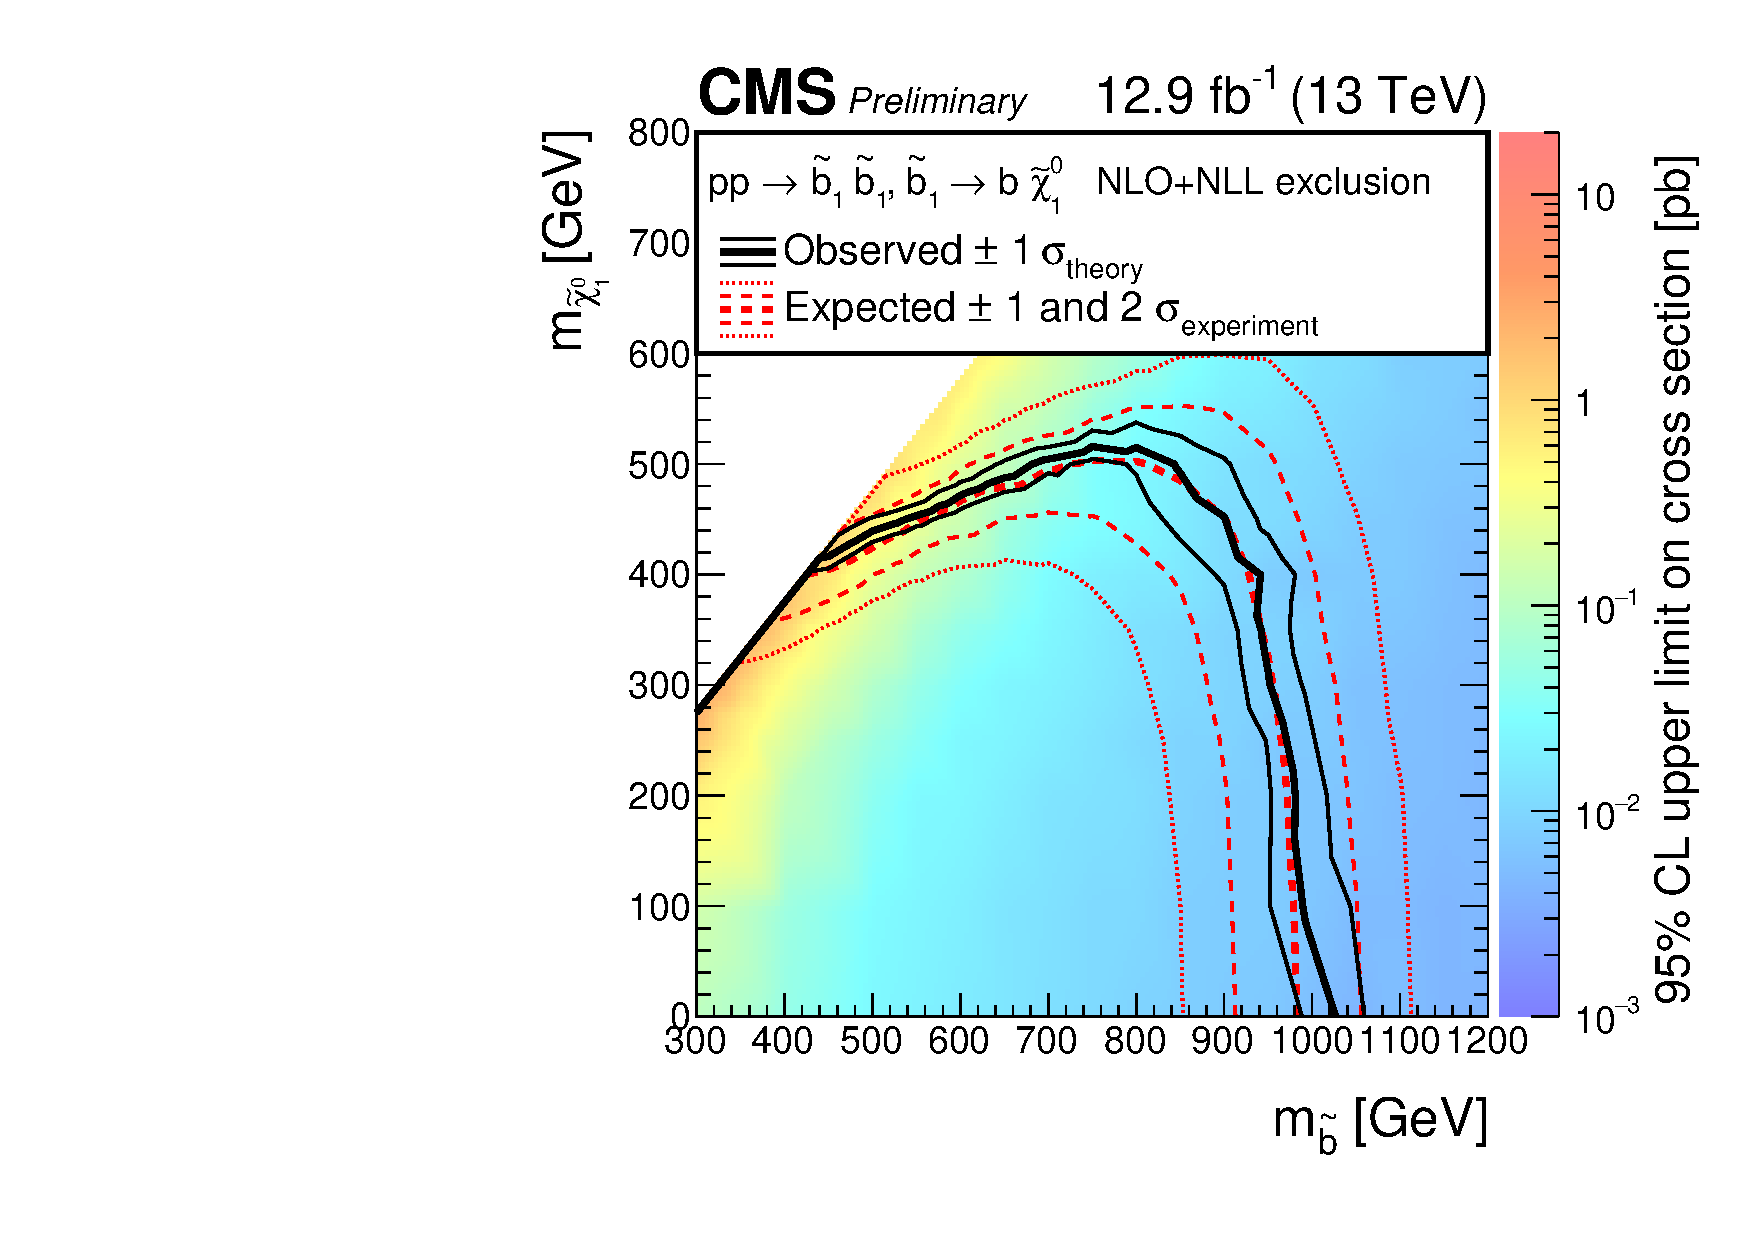
\includegraphics[width=0.45\textwidth]{figures/alphaT/limitPlanesNominal/SUS16T2bbXSEC} } ~~
    \subfigure[T2bb aggregate regions]{ 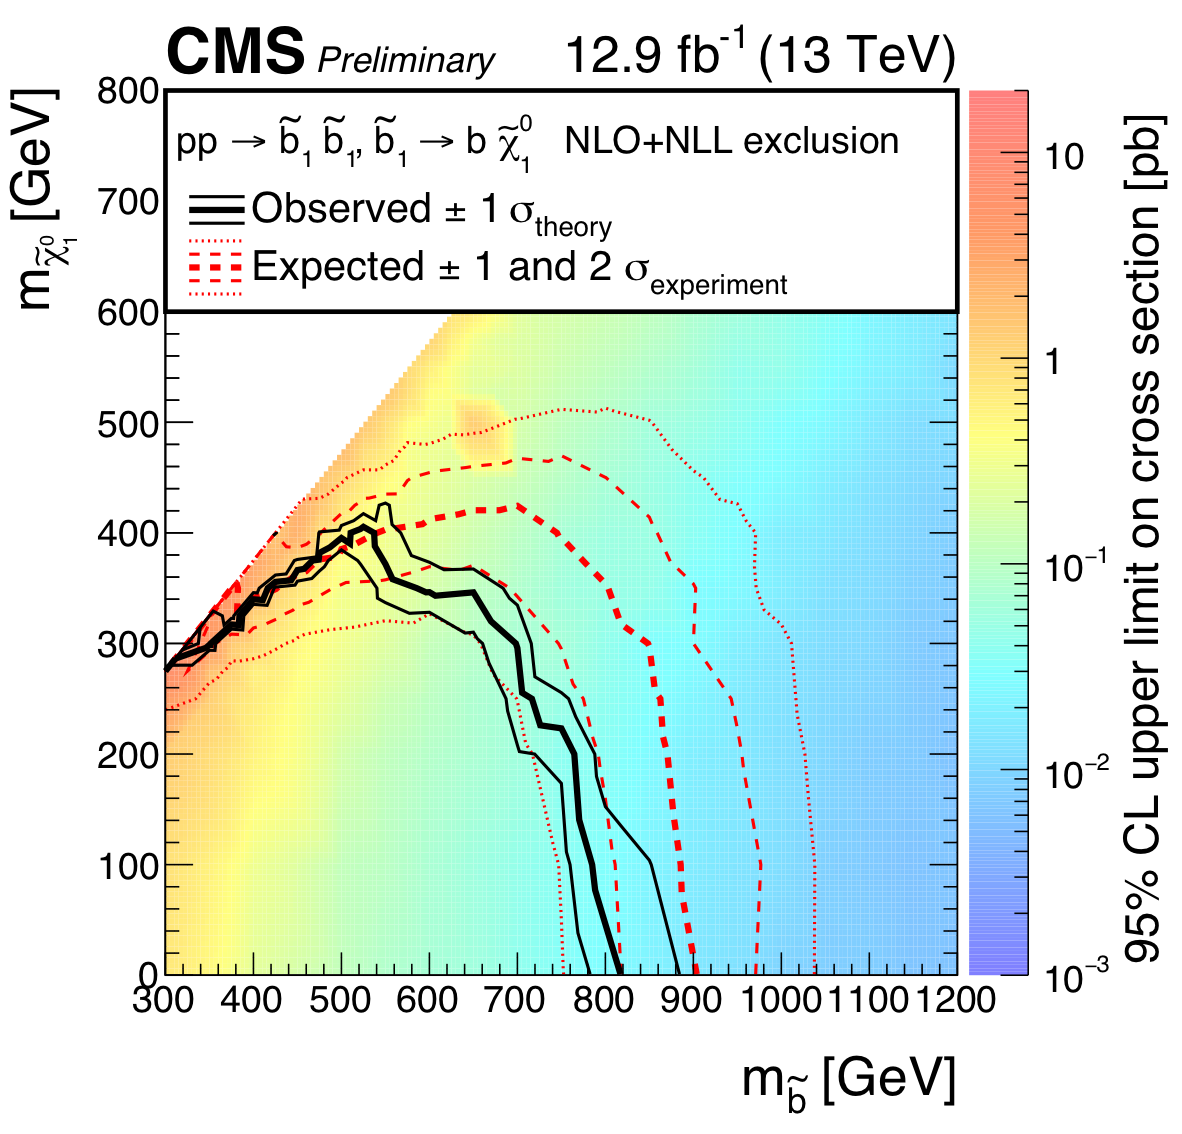
\includegraphics[width=0.45\textwidth]{figures/alphaT/limitPlanesAgg/SUS16T2bbXSEC} } \\
    \subfigure[T2tt full signal region]   { 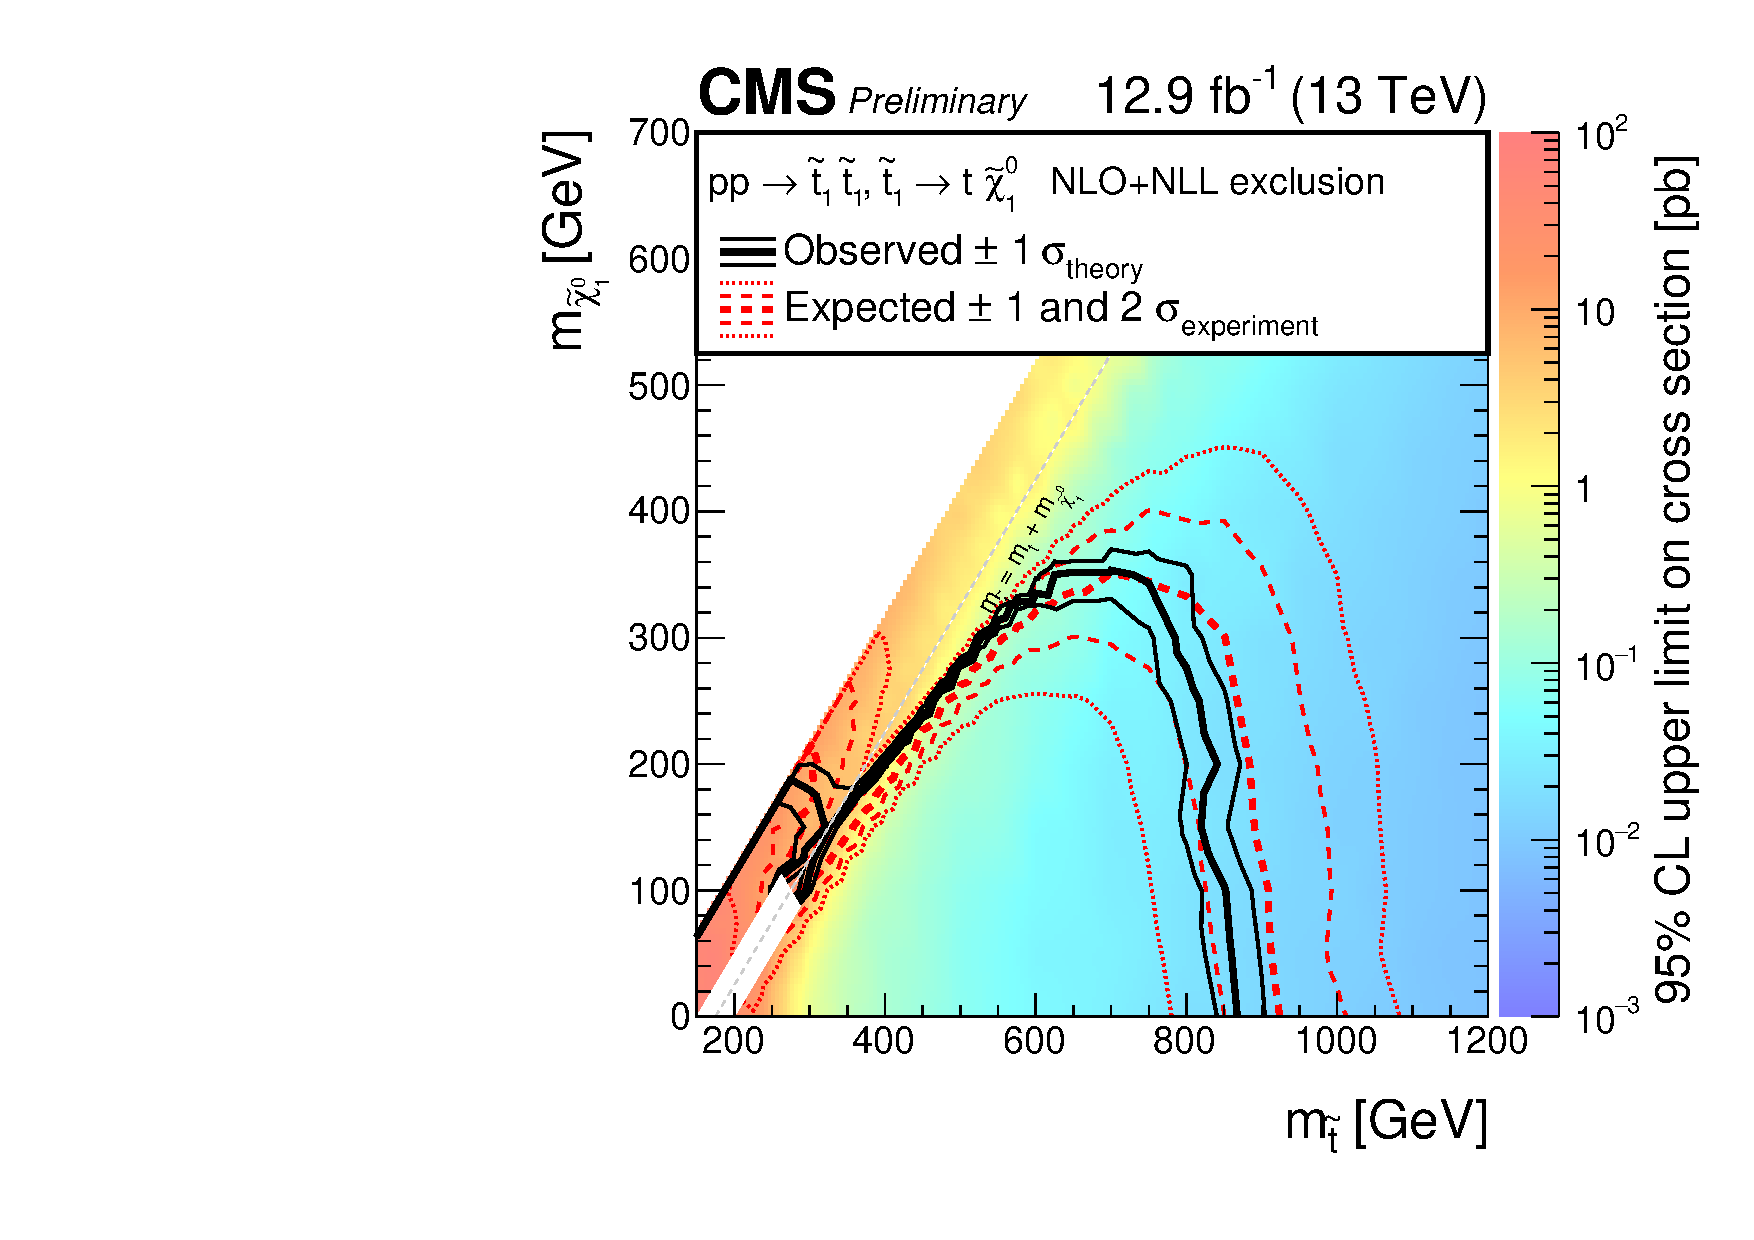
\includegraphics[width=0.45\textwidth]{figures/alphaT/limitPlanesNominal/SUS16T2ttXSEC} } ~~
    \subfigure[T2tt aggregate regions]{ 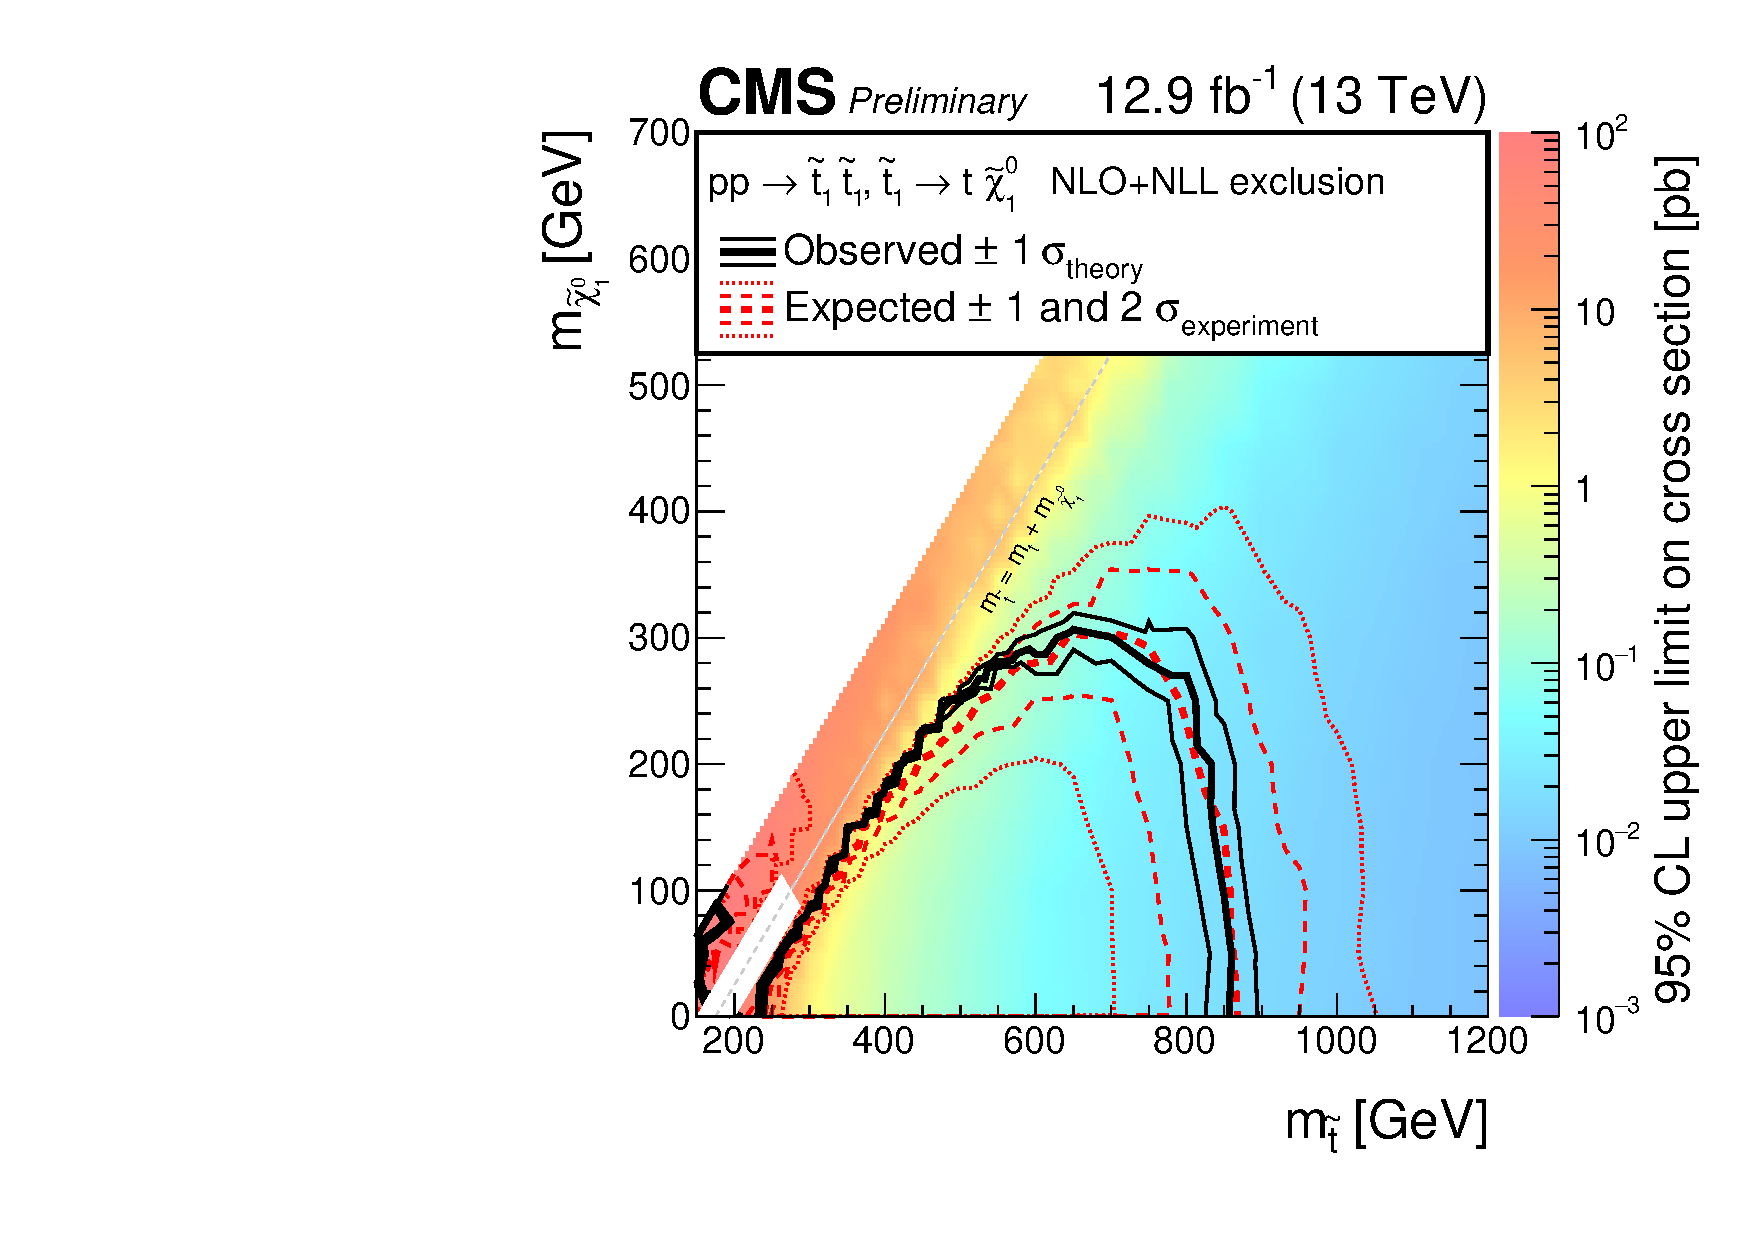
\includegraphics[width=0.45\textwidth]{figures/alphaT/limitPlanesAgg/SUS16T2ttXSEC} } \\
    \subfigure[T1bbbb full signal region]   { 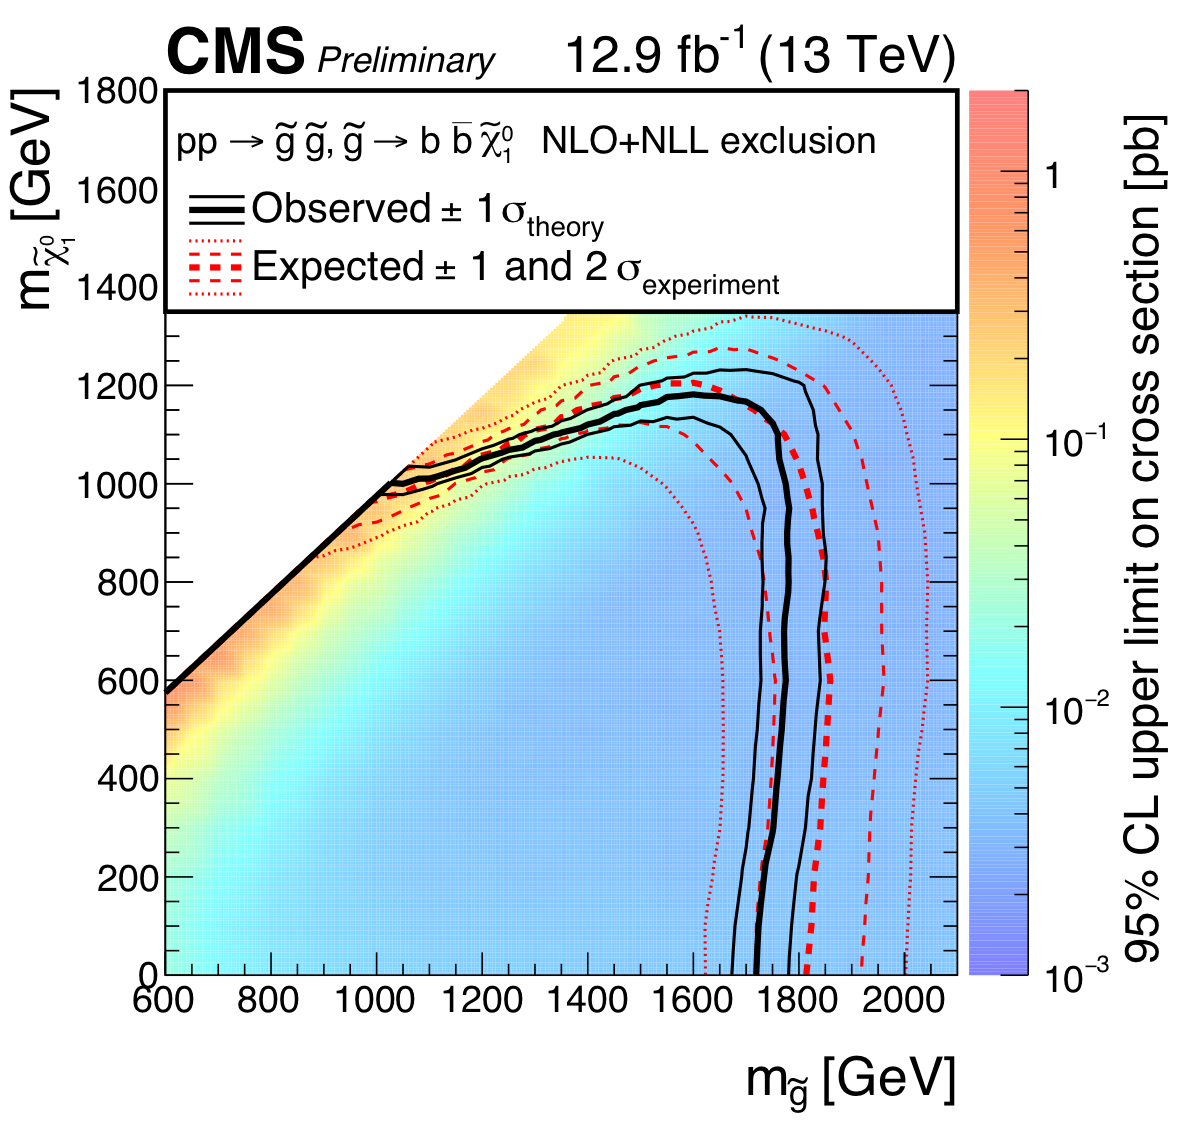
\includegraphics[width=0.45\textwidth]{figures/alphaT/limitPlanesNominal/SUS16T1bbbbXSEC} } ~~
    \subfigure[T1bbbb aggregate regions]{ 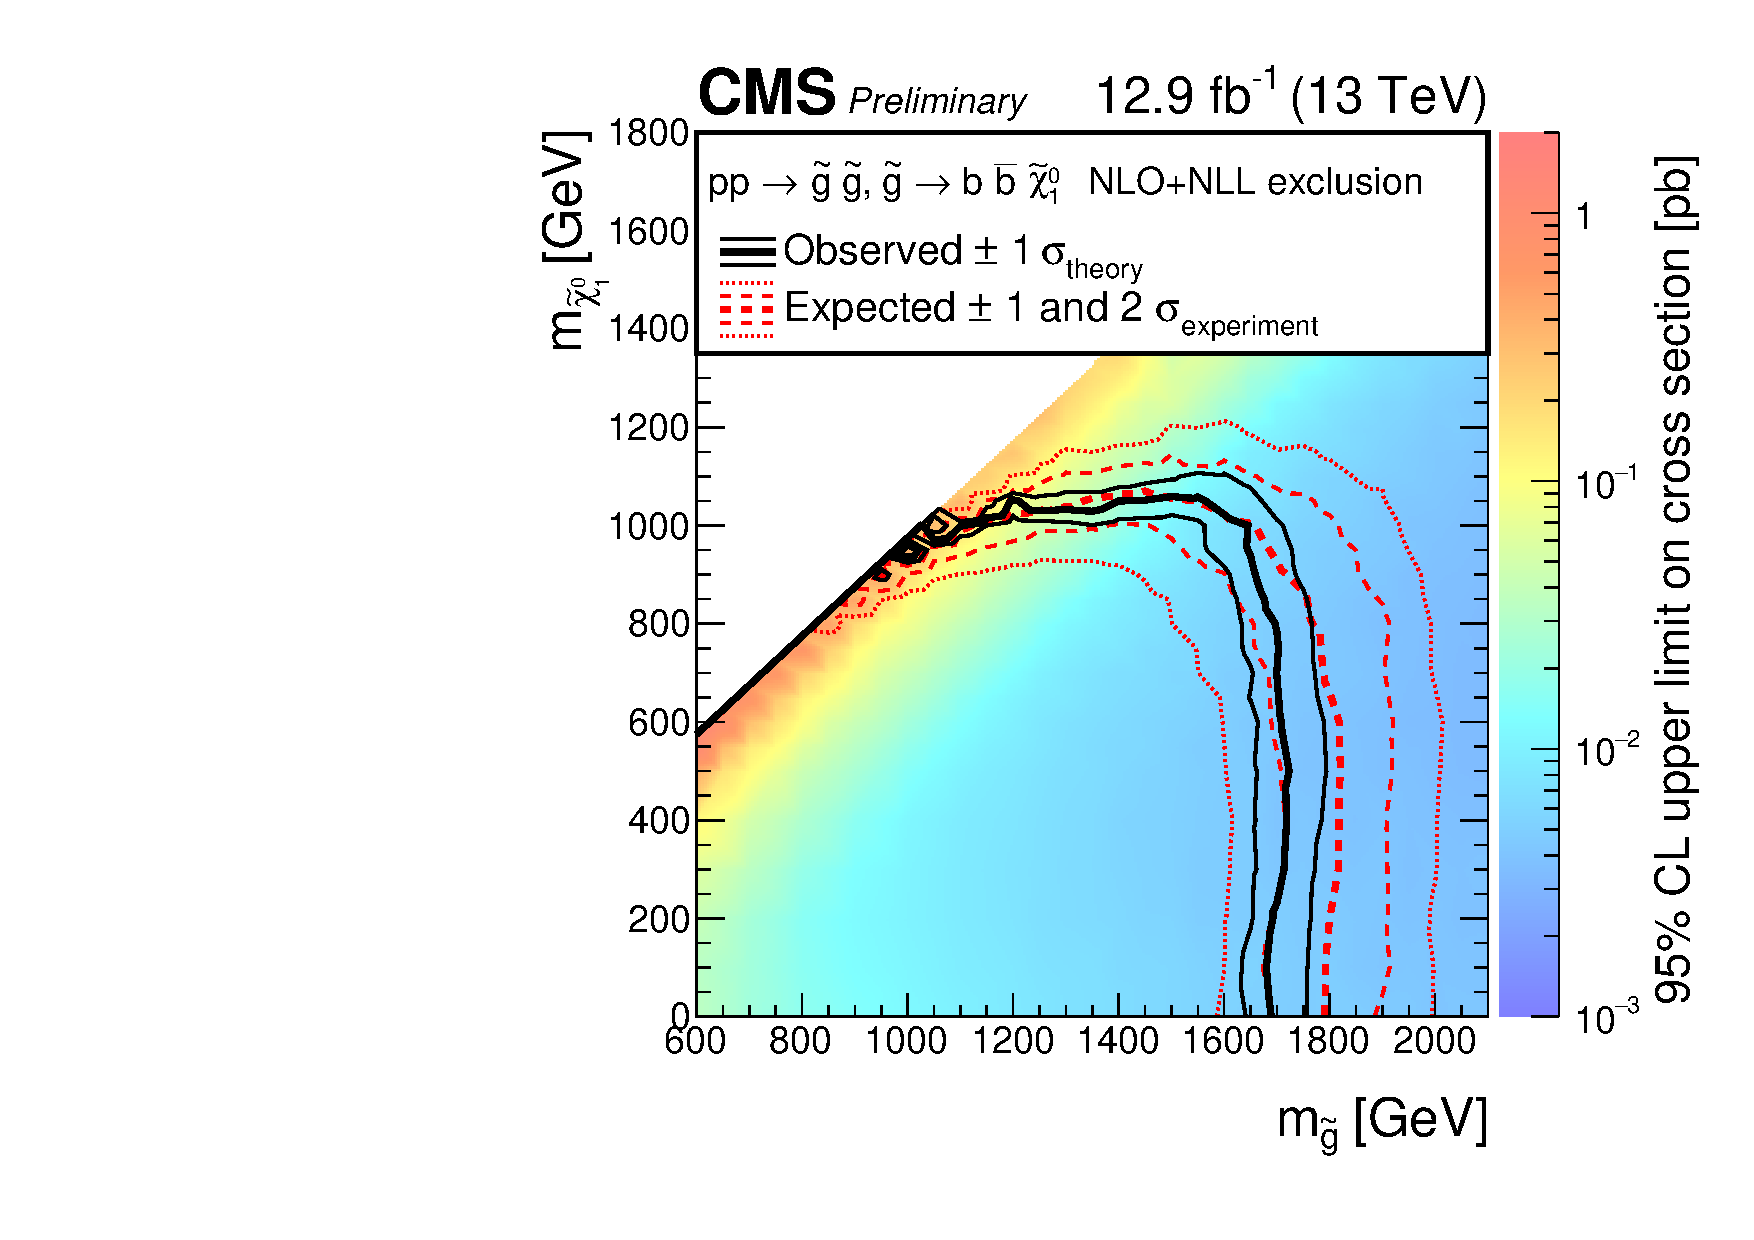
\includegraphics[width=0.45\textwidth]{figures/alphaT/limitPlanesAgg/SUS16T1bbbbXSEC} } \\
  \end{center}
\end{figure}

\subsection{Validation of the simplified likelihood}

The covariance and predictions of the aggregate regions for the \alphat analysis may then 
be used to validate the simplified likelihood. Figure~\ref{fig:likelihoodscan-alphaT} shows the value of $q(\mu)$ as a function of $\mu$ for 
a benchmark model which has substantial contribution in many different signal regions 
(T2tt mStop = , mLSP = ).The values when $q(\mu)$ is defined using the likelihood of Equation~\ref{eq:full-likelihood} 
are shown and compared with the same definition but assuming no correlations between the 
background yields by setting $V_{ij}=0$ for $i\neq j$. The results using the full likelihood (with aggregate regions and no signal systematics) 
used by the \alphat analysis are also shown. The simplified likelihood shows good agreement with the full likelihood 
while it is clear that ignoring the correlations results in a bias of the estimate of $\hat{\mu}$. 

\begin{figure}[hbt]
  \begin{center} 
   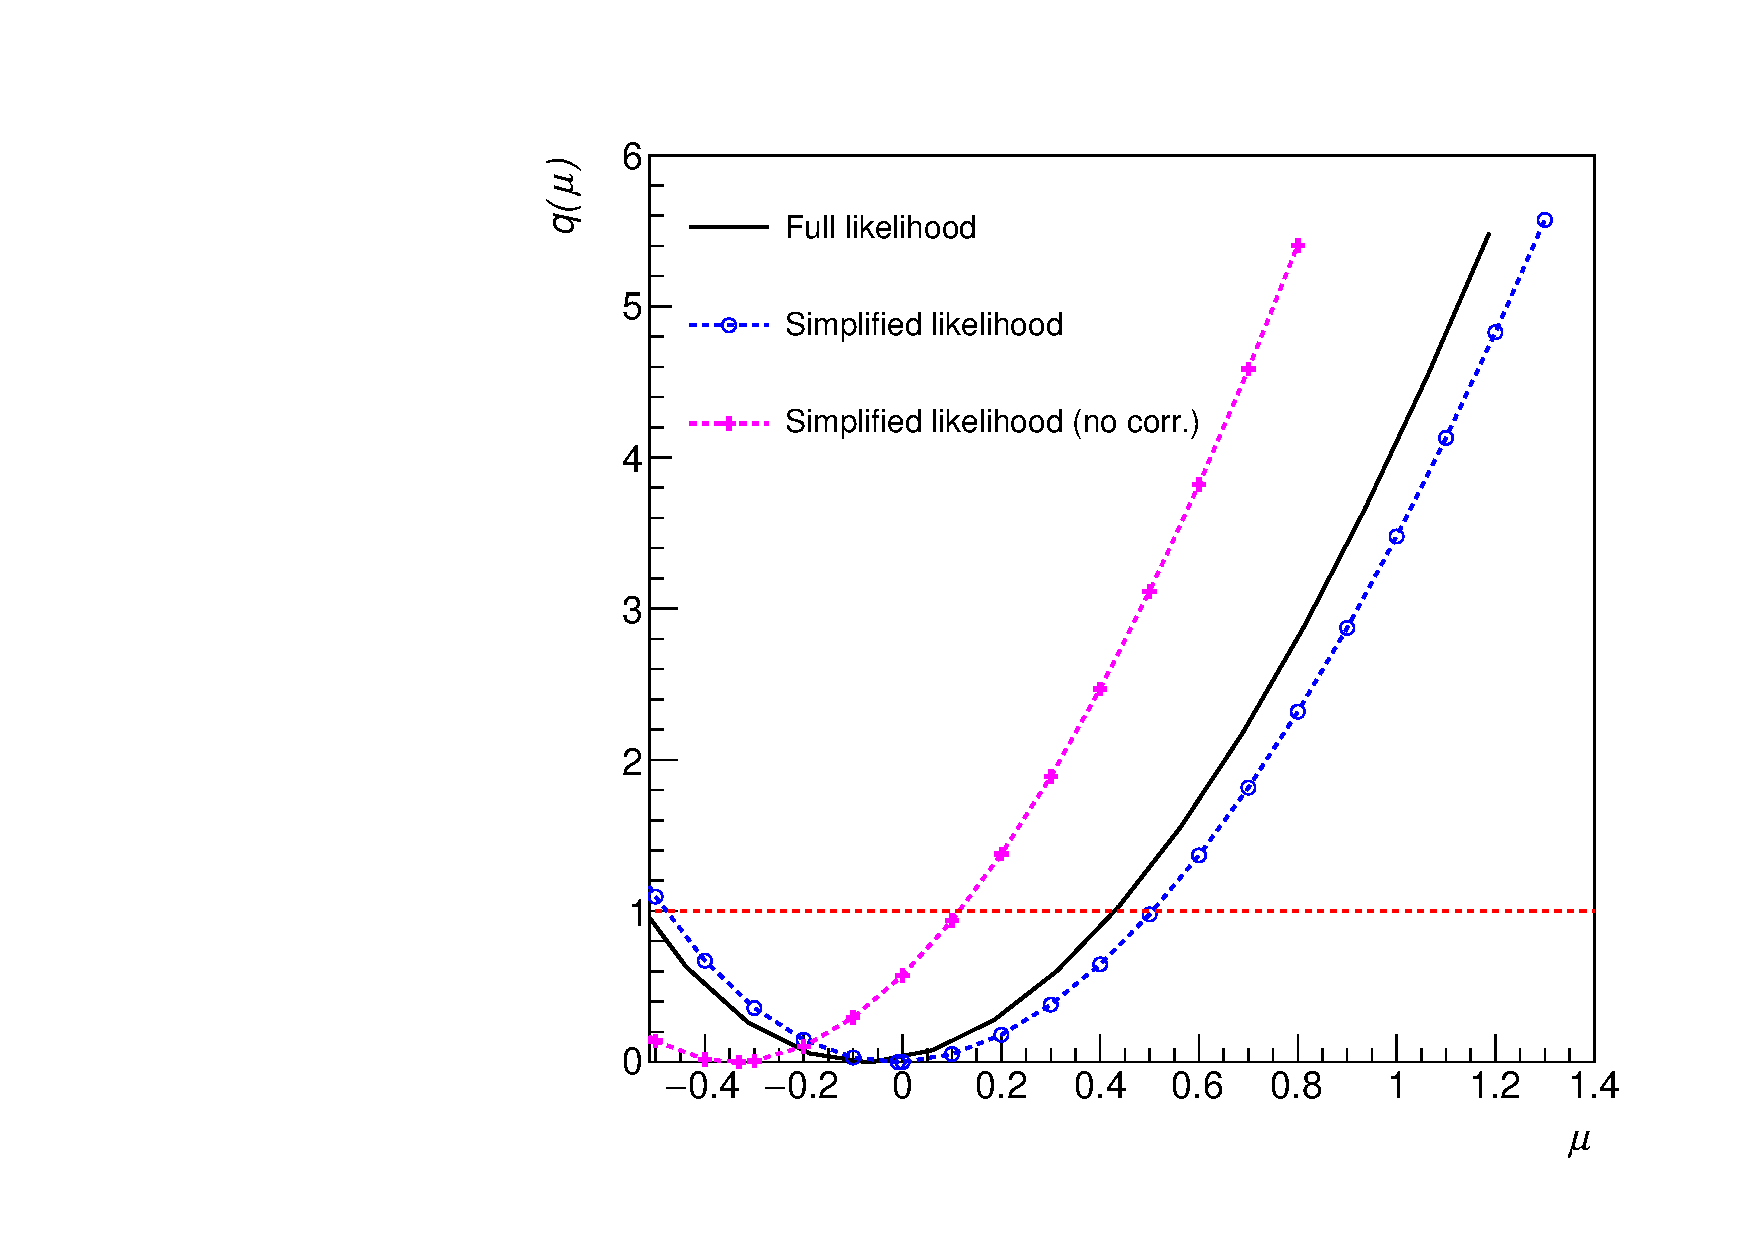
\includegraphics[width=1.5\cmsFigWidth]{figures/alphaT/rAT.pdf}
   \caption{The value of $q(\mu)$ for the \alphaT analysis defined using the simplified likelihood using the full covariance matrix (open blue points), assuming no correlations between the 
   background yields (open magenta crosses) and defined using the full likelihood (solid black line).}
   \label{fig:likelihoodscanAT} 
  \end{center}
\end{figure}

Finally, the limits across the full plane for a sample model (T2bb) are shown in Figure~{}.
In Figure~\ref{fig:limitPlanes} the ratio between the limit with the simplified and the full likelihood are shown.
The contours of $\mu=1$ excluded at $95\%$ for the full likelihood, the simplified likelihood
and the simplified likelihood where correlations are neglected are overlaid. When correlations
are considered the simplified and full likelihood provide comparable results, however, if 
these are neglected a significant bias is observed.

\begin{figure}[hbt]
  \begin{center} 
   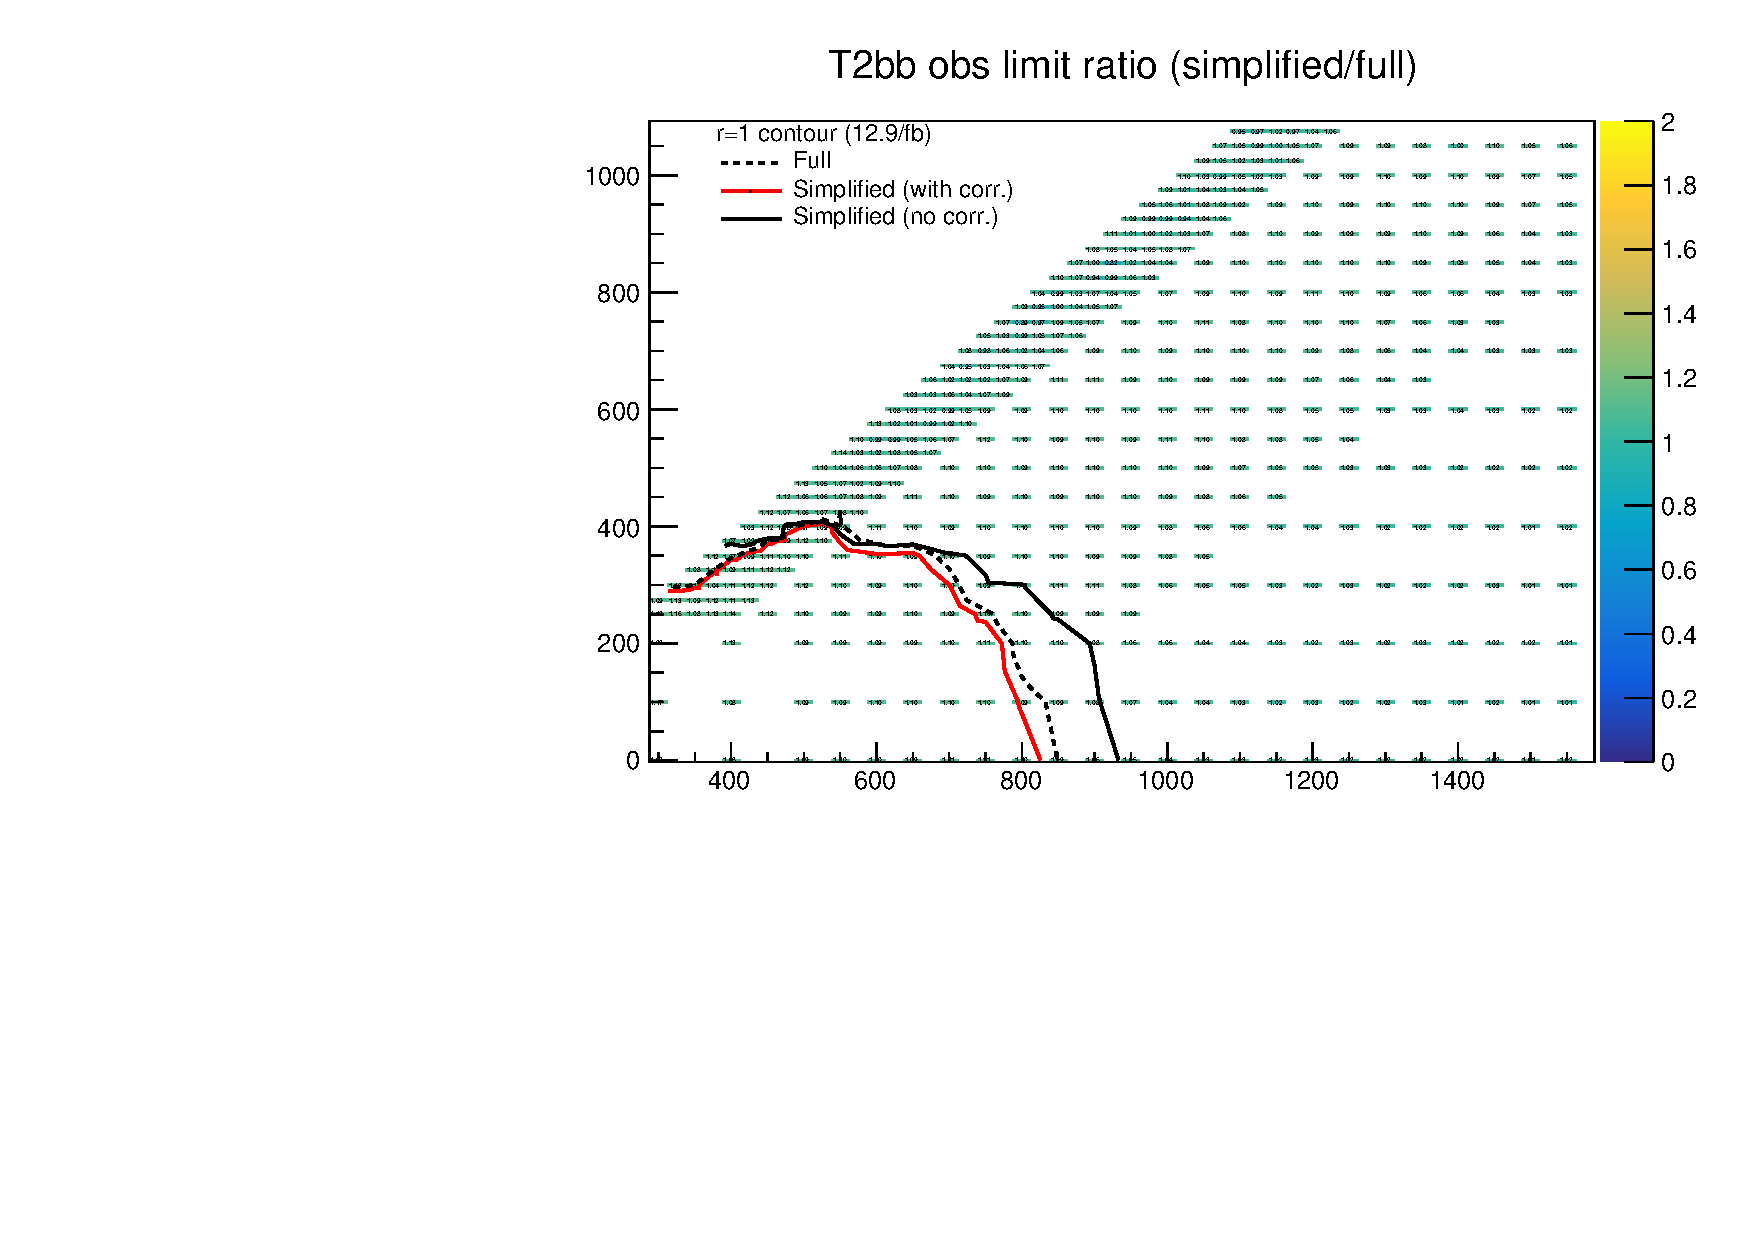
\includegraphics[width=1.5\cmsFigWidth]{figures/alphaT/full_T2bb_obs}
   \caption{Ratio of the $95\%$ upper limits for the simplified likelihood/full likelihood.
   The contour of $\mu=1$ for the simplified likelihood using the full covariance matrix (solid red line), 
   the simplified likelihood assuming no correlations between the background yields (solid black line) and the full
   likelihood (dotted black line) are overlaid.
   }
   \label{fig:limitPlanes} 
  \end{center}
\end{figure}
%%____________________________________________________________________________||






%%____________________________________________________________________________||

